\documentclass[12pt,table]{beamer}

\usepackage{ut-defense}
\usepackage{graphicx,caption}  % Required for including images
\usepackage{booktabs} % Top and bottom rules for tables
\usepackage{amssymb,amsthm,amsmath,bm}
\usepackage{exscale}
\usepackage{natbib}
\usepackage{tikz}
\usepackage{listings}
\usepackage{bm}
\usepackage{hyperref}
\usepackage{media9}
\usepackage{perpage}
\usepackage{cancel}
\usepackage[table]{xcolor}
\usepackage{wasysym}
\usepackage{array}
\usepackage{tabularx}
\usepackage{appendixnumberbeamer}
%\renewcommand{\CancelColor}{\color{red}}
\MakePerPage{footnote}
\setbeamercovered{transparent}

\newcommand{\etal}{\emph{et al.}}

% \AtBeginSection[]{
%   \begin{frame}
%   \vfill
%   \centering
%   \begin{block}{}
%     \vspace{.25cm}
%     \centering
%     \usebeamerfont{title}\insertsectionhead\par%
%     \vspace{.25cm}
%   \end{block}
%   \vfill
%   \end{frame}
% }
% \AtBeginSubsection[]{
%   \begin{frame}
%   \vfill
%   \centering
%   \begin{block}{}
%     \vspace{.25cm}
%     \centering
%     \usebeamerfont{title}\insertsectionhead:  \\\insertsubsectionhead\par%
%     \vspace{.25cm}
%   \end{block}
%   \vfill
%   \end{frame}
% }

% \usepackage{helvet}
% \renewcommand{\familydefault}{\sfdefault}
%  trim={<left> <lower> <right> <upper>}
\newcommand{\gke}{{\tt Gkeyll}}
\newcommand{\vpar}{{v_\parallel}}

\begin{document}

\title[DG Modeling of SMT Plasma Turbulence]{\LARGE Discontinuous Galerkin Modeling of Plasma Turbulence in a \\ Simple Magnetized Torus}%
\author[T. Bernard]{\large Tess Bernard}%
\date{Final Public Oral Defense \\ May 8, 2019}

\addtocounter{framenumber}{-1}
\begin{frame}[plain]
  \titlepage
\end{frame}

\begin{frame}{Outline}
    \tableofcontents
\end{frame}

\begin{frame}{Thesis research highlights}
\begin{itemize}
    \item Simulated a two-dimensional fluid model of blob turbulence with Helimak parameters using the DG code ArcOn and carried out theoretical analysis of instabilities in various limits.
    {\bf \item Used the plasma computational framework \gke\ to run continuum gyrokinetic simulations of the Texas Helimak
    \item Conducted extensive post-processing to analyze results.
    \item Carried out validation with experimental data of grounded and limiter-biasing simulations performed with \gke.}
    \item Contributed to implementation of a moment-conserving gyrokinetic Fokker-Planck collision operator in \gke.
\end{itemize}    
\end{frame}

\section[Background]{{\bf Simple magnetized torus experiments} and relevance to fusion devices}

\begin{frame}{Chasing a star:~clean energy via fusion}
\begin{minipage}{\linewidth}
    \begin{minipage}{.35\linewidth}
    \begin{figure}
        \centering
        %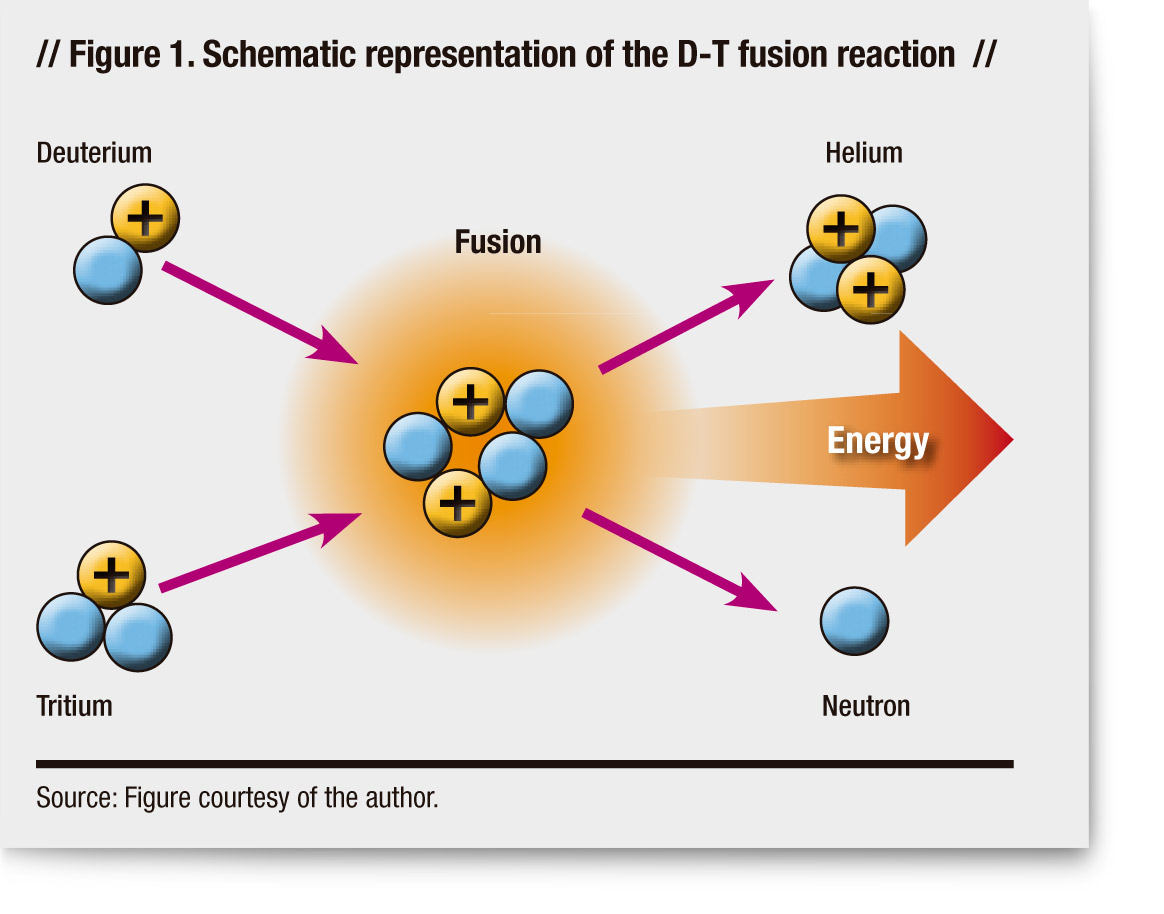
\includegraphics[width=\linewidth, clip, trim= 0cm 6cm 3cm 4cm ]{figs/fusion_dt_ENG.jpg}
        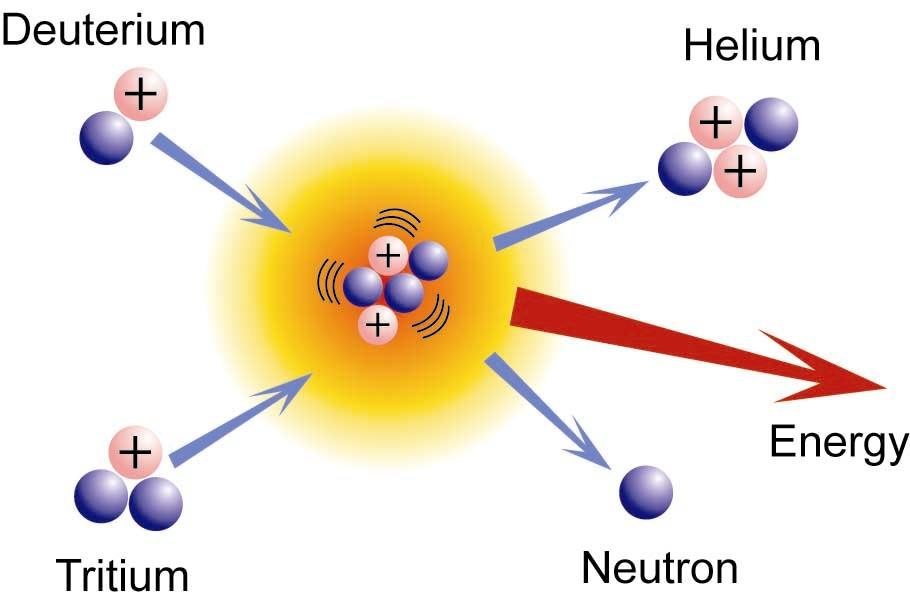
\includegraphics[width=\linewidth]{figs/fusion.jpg} \\
        \tiny From universetoday.com
    \end{figure}%
    \end{minipage}%
    \begin{minipage}{.65\linewidth}
    \begin{itemize}
        \footnotesize
        \item Naturally occurring process in stars (made of \textbf{plasma})
        \item Requires temperatures $\sim$6x hotter than sun's core to produce fuel on faster time scale (10~million K)
        \item Must satisfy \emph{Lawson's Criterion}:
        $n_p \tau \geq 1.4 \times 10^{20}$ s m$^{-3}$ (D-T plasma)
        \item \textbf{Magnetic confinement fusion}:~use strong magnetic fields in toroidal configurations to contain the plasma%, i.e.~tokamak or stellarator. 
    \end{itemize}%
    \end{minipage}
\end{minipage}
    \vfill
    \begin{minipage}{.3\linewidth}
        \begin{figure}
        \centering
        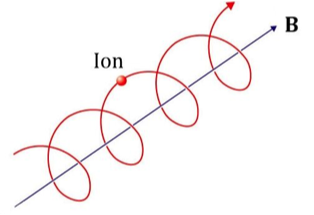
\includegraphics[width=\linewidth]{figs/cyclotron_motion.png} \\
        \tiny From eurofusion.com
    \end{figure}
    \end{minipage}
    \hfill
    \begin{minipage}{.65\linewidth}
    \begin{figure}
        \centering
        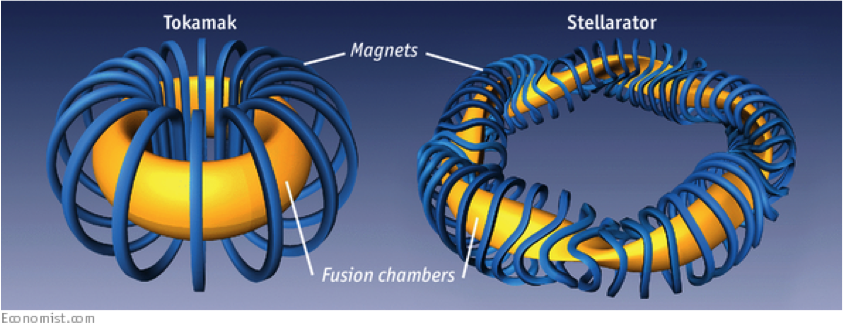
\includegraphics[width=.9\linewidth,clip, trim = .5cm .5cm .5cm 0cm]{figs/tok-stell.png} \\
        \tiny From economist.com
        \label{fig:my_label}
    \end{figure}
    \end{minipage}
    % Possible questions: 
    % What is sun/star temperature? 
\end{frame}

\begin{frame}{Tokamak:~the fusion donut}
\begin{minipage}{.6\linewidth}
    \begin{figure}
        \centering
        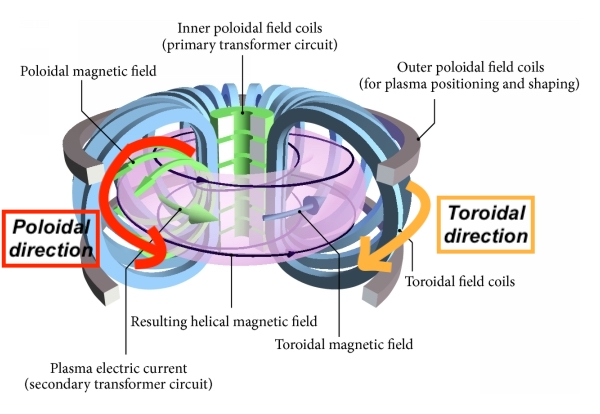
\includegraphics[width=\linewidth]{figs/tokamak.jpg} \\
        \tiny From Li \etal\ (2014)
        % http://dx.doi.org/10.1155/2014/940965
        \label{fig:my_label}
    \end{figure}
    Plasma scientists use computational tools extensively to better understand plasma instabilities in tokamaks. 
\end{minipage}
%\hfill
\begin{minipage}{.35\linewidth}
\begin{figure}
    \centering
    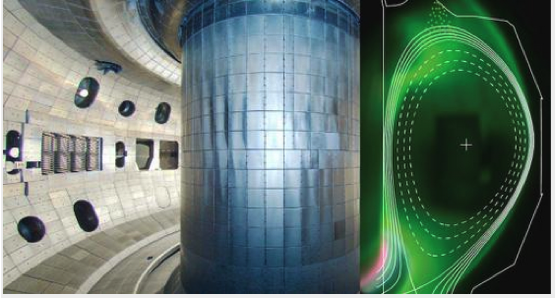
\includegraphics[width=1.2\linewidth]{figs/diii-d.png}\\
    \tiny DIII-D tokamak. Image credit: General Atomics and Steve Allen (LLNL).
\end{figure}%
\vspace{-1cm}
\begin{figure}
    \centering
    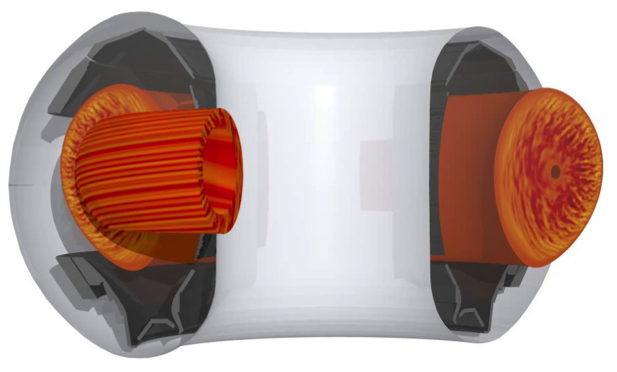
\includegraphics[width=1.2\linewidth]{figs/gene.png} \\
    \tiny Core simulation with GENE. Image credit: GENE development team.
\end{figure}
\end{minipage}
% or include cartoon on this page
\end{frame}

\begin{frame}{Boundary plasma plays key role in confinement}
    \begin{minipage}{.4\linewidth}
    % \begin{figure}
    %     \centering%
    %     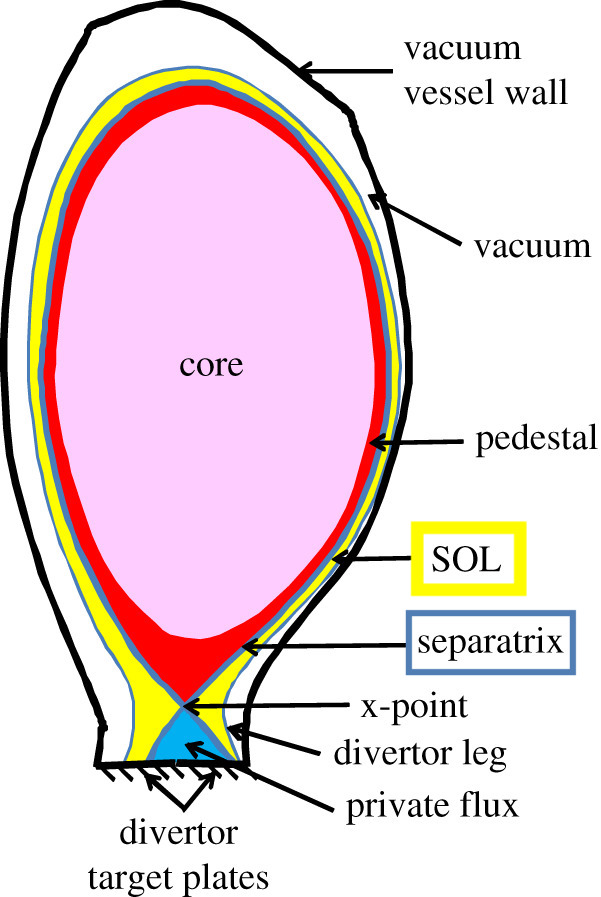
\includegraphics[width=\linewidth]{figs/rsta20170435f06.jpg} \\
    %     \scriptsize Tokamak cross section from H.~Wilson (2019). %https://doi.org/10.1098/rsta.2017.0435}
    % \end{figure}
    \vspace{-1cm}
    \begin{figure}
        \centering%
        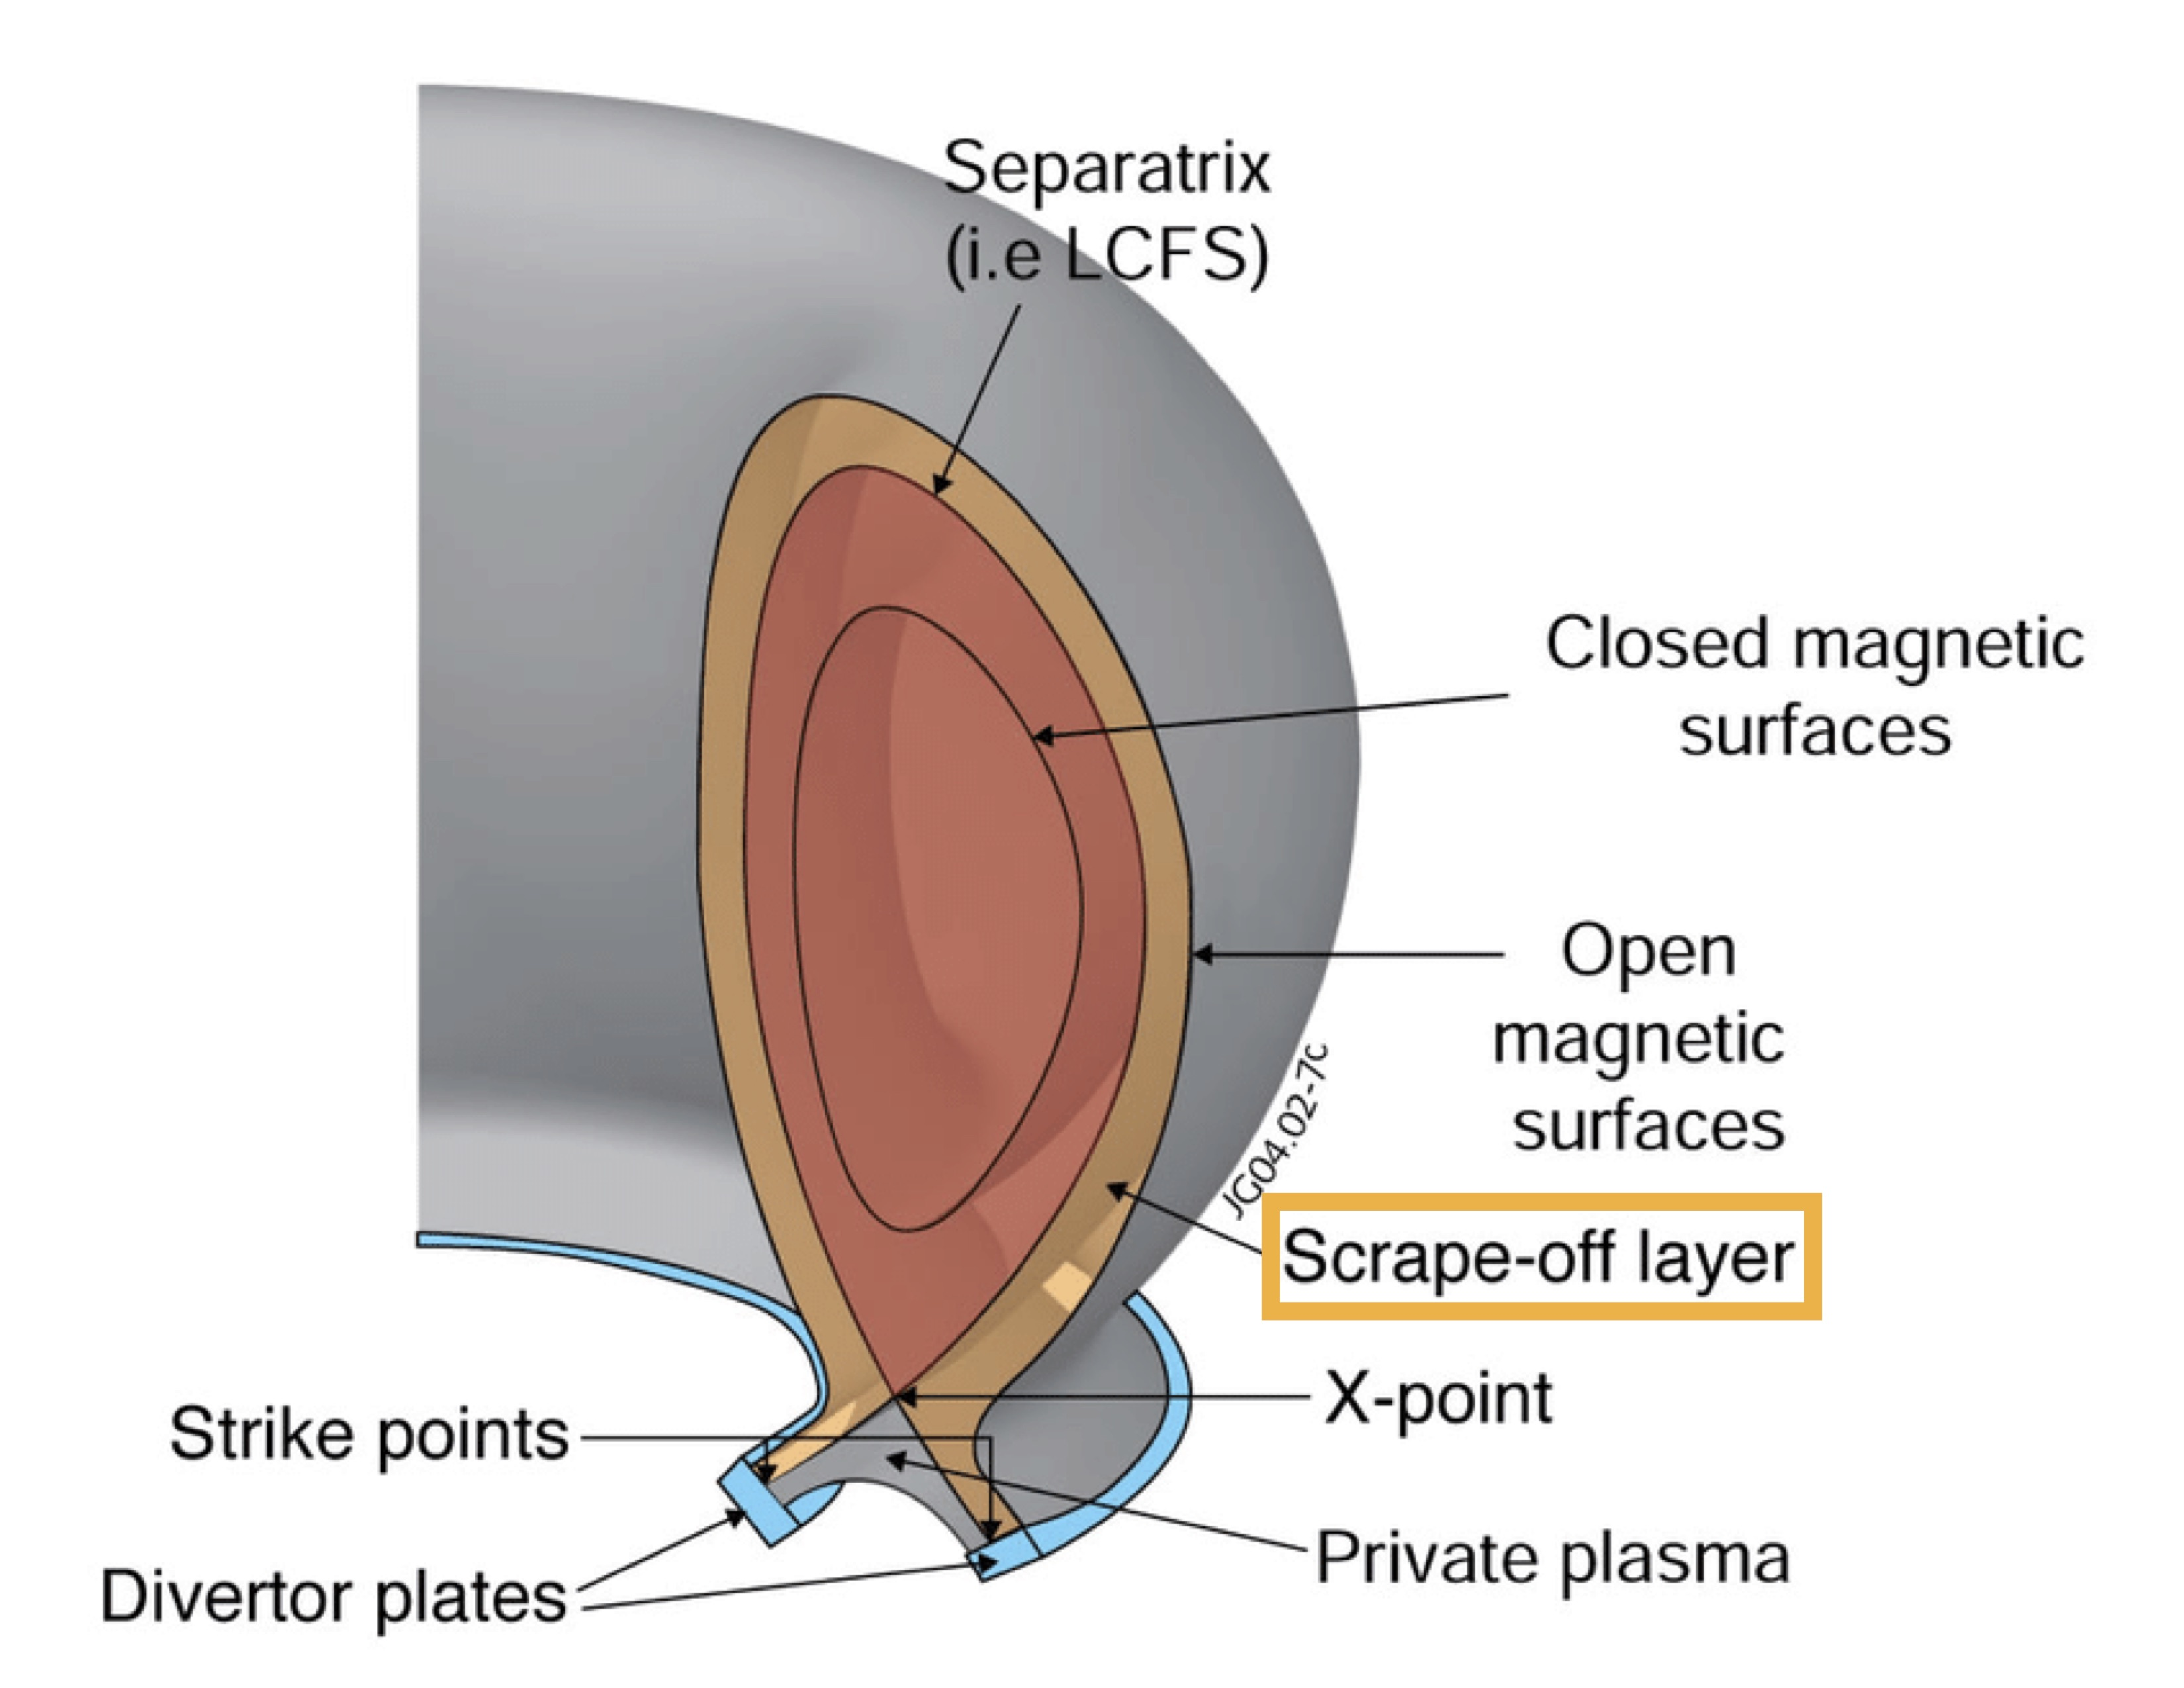
\includegraphics[width=1.2\linewidth,clip,trim = 5cm 0cm 0cm 0cm]{figs/sol-labeled.jpg} \\
        \tiny From C.~Theiler (2011). %https://doi.org/10.1098/rsta.2017.0435}
    \end{figure}
    \end{minipage}%
    \begin{minipage}{.6\linewidth}%
        \begin{itemize} \footnotesize
        \item The tokamak \textbf{\textcolor{UT_orange}{scrape-off layer}} (SOL) lies outside the last closed magnetic flux surface and contains magnetic field lines that connect to the wall.
        \item Characterized by heat and particle flow along magnetic field lines and turbulent transport across field lines.
        \item Balance between parallel and cross-field transport determines how particles and heat are exhausted to divertor plates.
        \item Uncertainty in how SOL heat flux width scales with machine size.
        \end{itemize}
    \end{minipage}
\end{frame}

\begin{frame}{Intermittent turbulent structures observed in SOL}
    \begin{minipage}{.65\linewidth}
    \begin{itemize} \footnotesize
        \item Coherent turbulent structures called \textbf{\textcolor{UT_orange}{blobs}} form at the edge of the core plasma and have higher density than surrounding plasma
        \item Blobs become polarized by curvature and $\nabla B$ forces and drift radially towards the wall due to $E \times B$ force.
        \item Could potentially damage plasma-facing components and add impurities {\large \textcolor{red}{\frownie{}}}
        \item Could diffuse heat load to divertor plates {\large\textcolor{green}{\smiley{}}}
    \end{itemize}%
    \end{minipage}
    \begin{minipage}{.3\linewidth}
    \begin{figure}
        \centering
        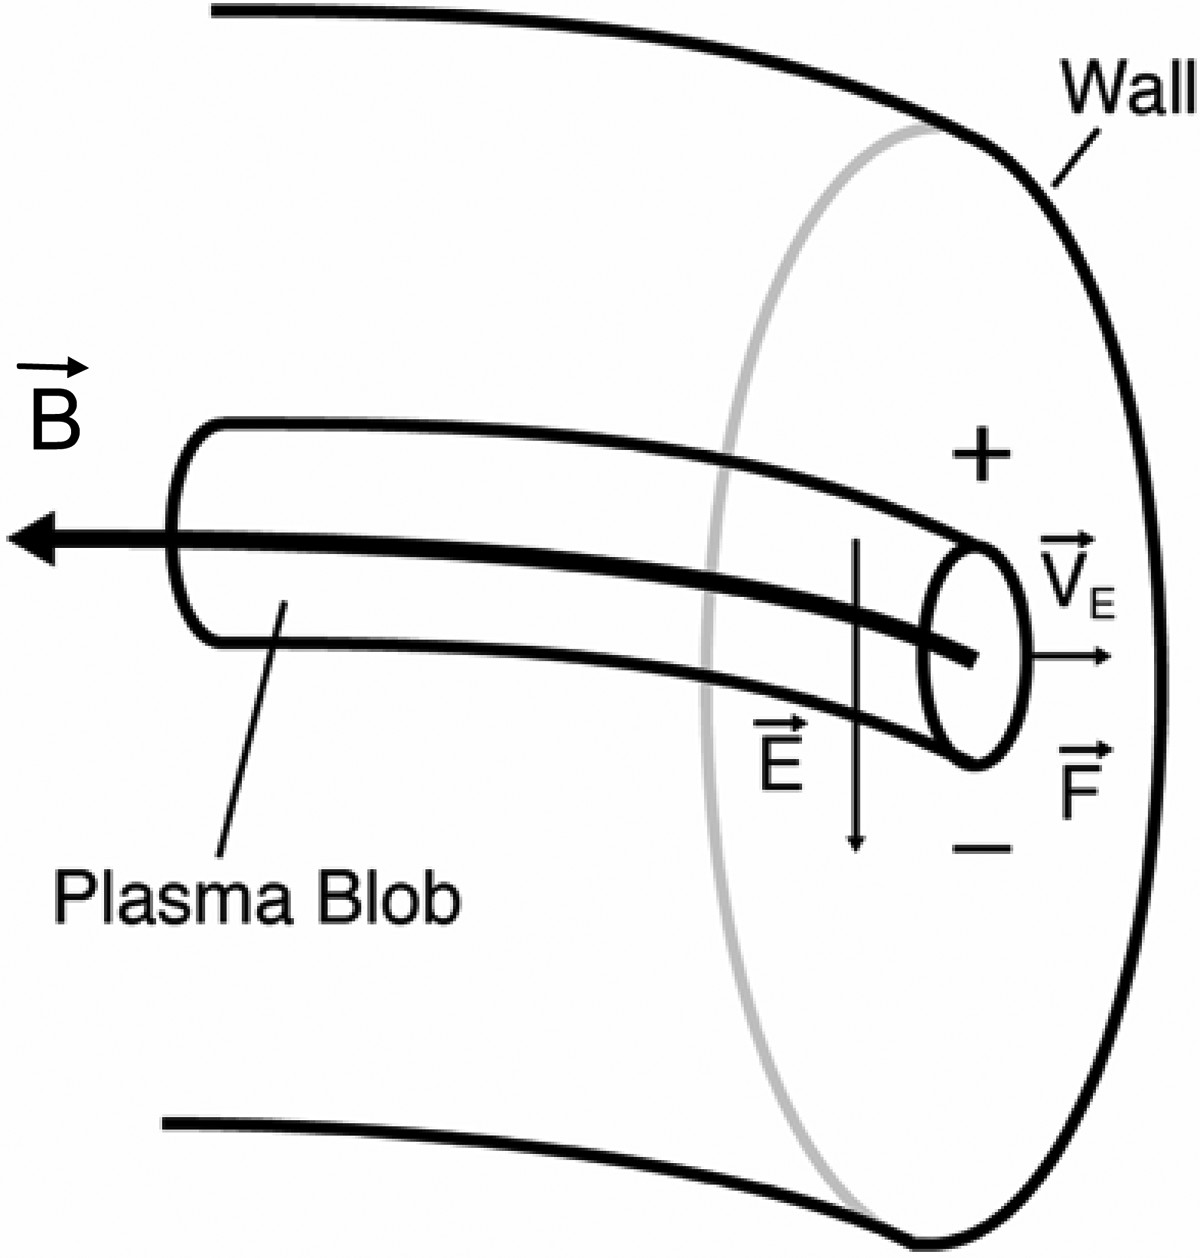
\includegraphics[width=.9\linewidth]{figs/plasma-blob.jpeg} \\
        \tiny From D'Ippolito \etal\ (2011)
    \end{figure}
    \end{minipage}%
    \vfill
    \begin{minipage}{0.63\linewidth}
        \centering
        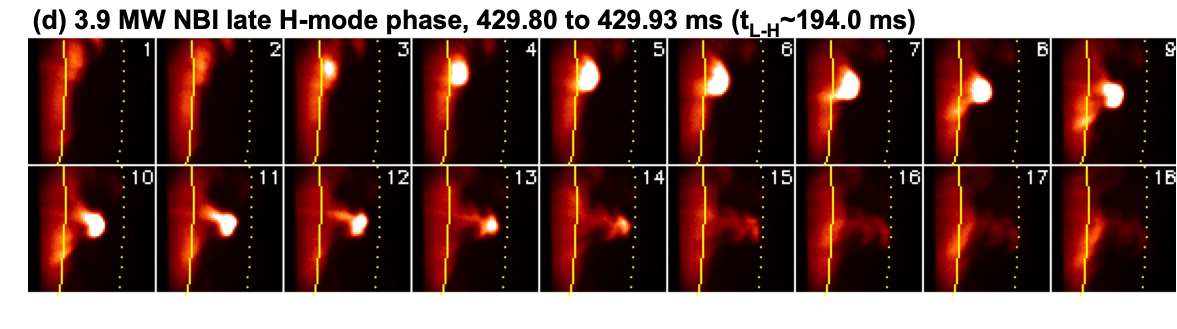
\includegraphics[clip, trim=.25cm .2cm 0cm .6cm, width=\linewidth]{figs/nstx-blob.png}
    \end{minipage} \hfill
    \begin{minipage}{0.35\linewidth}
        \scriptsize Blobs in NSTX SOL from GPI diagnostic. From Maqueda, R.~J. \etal\ (2011).
        \label{fig:nstx-blob}
        \end{minipage}%
\end{frame}

\begin{frame}{SMTs are testbeds for tokamak-SOL models}
    \begin{minipage}[t]{0.45\linewidth}
    \begin{itemize} \scriptsize
        \item Simple magnetized torus (SMT) devices are experimental realizations of infinite sheared cylinder
        \item SMTs allow investigation of SOL-like turbulence in simple geometry
        \item Plasma properties similar to tokamak SOL: bad curvature, open-field lines, large intermittent fluctuations
        \item Dimensionless parameters similar to tokamak-SOL
    \end{itemize}
    \begin{center}
        \tiny
        %\vspace*{-.25cm}
        \begin{tabular}{c|c|c}
            Parameter & Helimak & DIII-D SOL \\ \hline 
            $\rho_s/L_n$ & 0.2 & 0.05 \\
            $L_c$ & 50 m & 40 m\\
            $\beta$ & $4 \times 10^{-5}$ & $3 \times 10^{-4}$ \\
            $v_D/c_s$ & 0.2 & 0.06 \\
            $L_c/\lambda_{ee}$ & 0.1 & 0.02 \\
            $\Delta n/n$ & 0.4 & 0.3 \\
        \end{tabular}
        \end{center}
        \begin{center}
        \vspace*{-.25cm}
        \tiny Table: Williams, C. Ph.D. Thesis. UT Austin, 2017.
    \end{center}
    \end{minipage}%
    \begin{minipage}[t]{0.5\linewidth}
    \vspace{-.25cm}
        \begin{figure}
        \captionsetup{width=.6\linewidth}
        \centering
        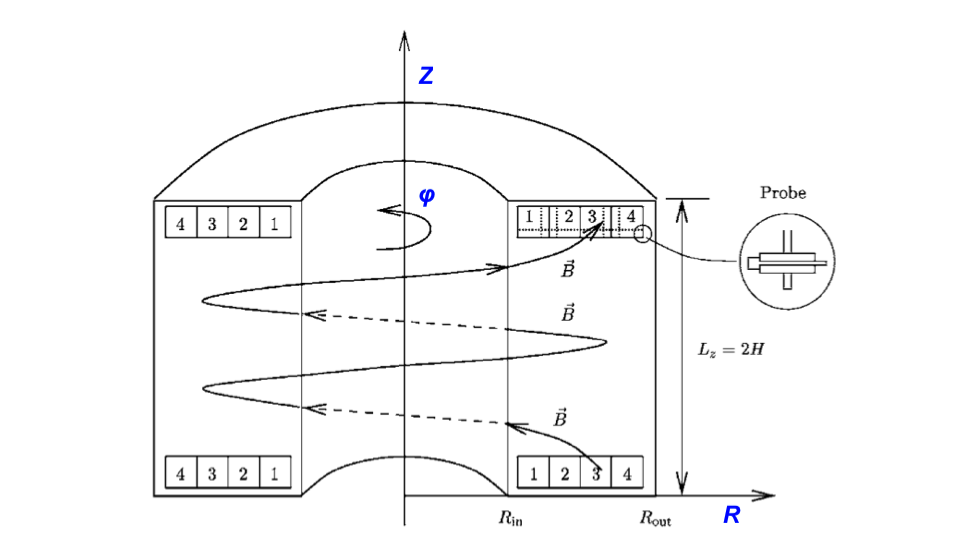
\includegraphics[width=1.3\linewidth,clip,trim=1cm 0cm 0cm 0cm]{figs/heli-cross-sec1.png} \\
        \tiny Schematic of \textbf{Texas Helimak} (above). Adapted from Perez \etal\ (2006). Toroidal coordinates for comparison (below). 
        \hfill
        \begin{figure}
            \centering
        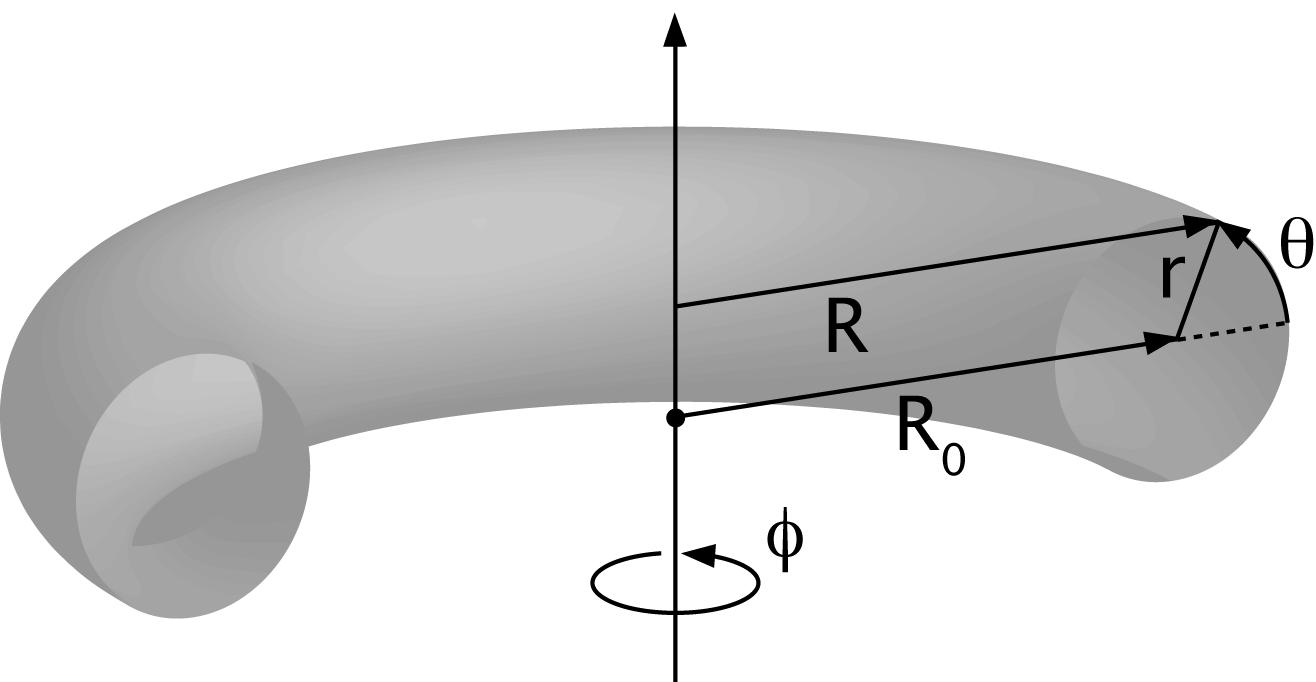
\includegraphics[width=.6\linewidth]{figs/Toroidal_coordinates.png}
        \end{figure}
    \end{figure}
    \hfill
    \end{minipage}%
\end{frame}

% \begin{frame}{SMTs are testbeds for tokamak-SOL models}
% \begin{figure}
% \begin{minipage}{.65\linewidth}
%         \centering
%         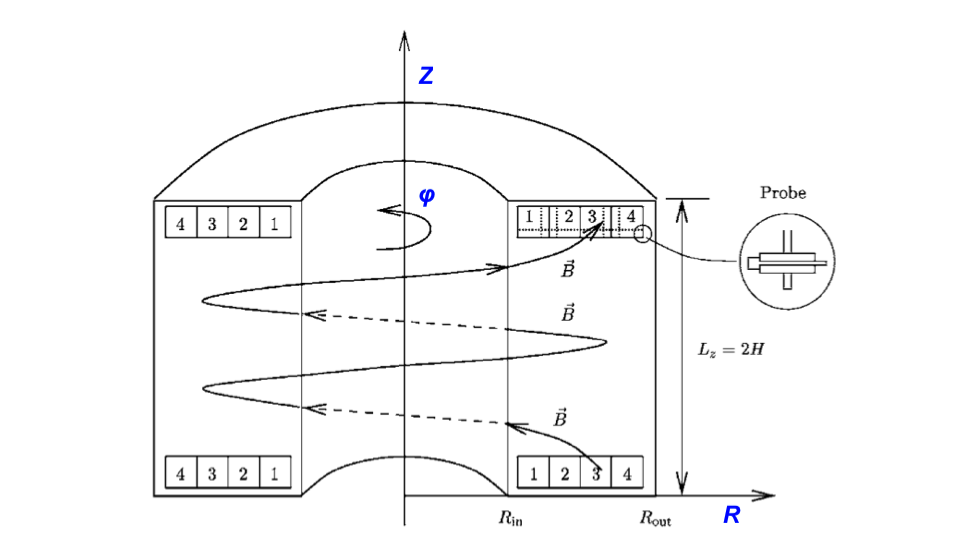
\includegraphics[width=\linewidth, clip, trim= 2cm .2cm 2cm .3cm]{figs/heli-cross-sec1.png}
%         \label{fig:heli-cs1}
% \end{minipage}
% \begin{minipage}{.30\linewidth}
% \vspace{2cm}
% \caption{Schematic of the Texas Helimak}
% \end{minipage}
%     \end{figure}%
%     \begin{itemize} \scriptsize
%         \item Simple magnetized torus (SMT) devices are experimental realizations of sheared cylinder
%         \item Allow investigation of SOL-like turbulence in simple geometry:
%         $R$ is tokamak major radius, $\varphi$ is toroidal angle and $Z$ is like poloidal angle
%         \item Plasma properties similar to tokamak SOL: density, temperature, collisionality, magnetic field strength, sheath physics
%         \item Dominant instabilities: \textbf{interchange} (Rayleigh-Taylor-like) from field-line curvature and \textbf{drift-wave} from density gradient
%     \end{itemize}
% \end{frame}

\begin{frame}{Texas Helimak\footnote{\scriptsize Gentle and He (2008); Gentle \etal\ (2010); Gentle \etal\ (2014)} is useful for code validation}
    \begin{minipage}{0.55\linewidth}
        \begin{itemize} \footnotesize
        \item Ion species: He$^+$, Ne$^+$, {\bf Ar$^+$}
        \item Injection of RF waves near electron cyclotron frequency sustains plasma
        %Power is absorbed at upper hybrid resonance
        \item Magnetic field line connection length depends on resistance in the vertical field coils
        \item Bias voltage applied to end plates to study effect of velocity shear on turbulence
        \item 500+ Langmuir probes, including baffled probes that directly measure plasma potential $\phi$
        \item Extensive diagnostics and simple geometry facilitate comparison with numerical models.
        \end{itemize}
    \end{minipage}%%
    \hfill
    \begin{minipage}{0.45\linewidth}
        \centering
        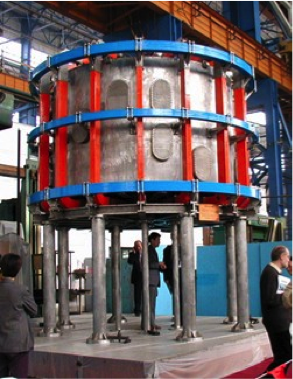
\includegraphics[width=.5\linewidth]{figs/heli-photo.png} \\
        \smallskip
        \begin{minipage}{.6\linewidth}
        \centering
            \tiny Photo of Helimak (top) and cutaway of vacuum vessel with $B$ field lines drawn in (bottom)
        \end{minipage} \\
        \smallskip        
        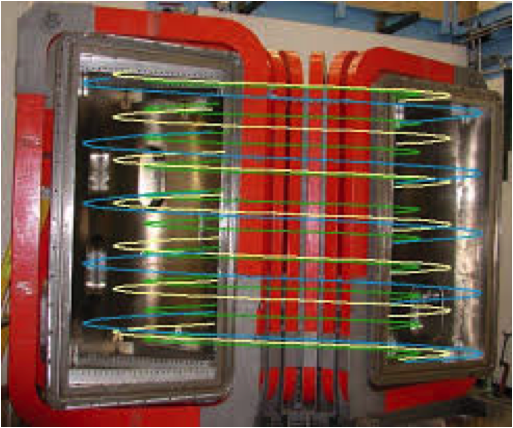
\includegraphics[width=.65\linewidth]{figs/heli-cross-sec2.png}
    \end{minipage}
\end{frame}

\section[Numerical modeling]{Numerical modeling and the {\bf discontinuous Galerkin (DG)} method}

\begin{frame}{Outline}
    \tableofcontents[currentsection] 
\end{frame}

\begin{frame}{Which numerical model is best for SMT or SOL plasmas?}
% add table as in USD presentation (fluid transport, fluid turbulence, gyrokinetic, full Vlasov)
% what is difference between transport and turbulence codes, what is ArcOn? 
    \begin{center}
    \footnotesize
        \begin{tabular} {|>{\centering\arraybackslash}m{5cm}| >{\centering\arraybackslash}m{5cm}|}
            \hline
            \rowcolor{myteal!40}
            \textbf{Fluid Models} & \textbf{Kinetic Models} \\ \hline
            Approximate ions and electrons 
            as two continuous fluids
            & Treat ions and electrons as particles, 
            tracking location and velocity \\ \hline
            Evolve various fluid properties \newline ($n$, $T$, $V$)
            & Evolve particle distribution function $f$ (Boltzmann eqn.) \\ \hline
            3 spatial dimensions $+$ time &
            3 spatial dimensions $+$ 3 velocity dimensions + time \\ \hline
            Computationally cheaper, may miss physics if plasma not sufficiently collisional &
            Comprehensive but computationally expensive \\ \hline
        \end{tabular}
    \end{center}
    % Note that there is a variety of fluid models that range from simple to very complete.
    \centering
    \begin{minipage}{.8\linewidth}
        \small
        \emph{Until recently, most SOL modeling has been with fluid codes, but kinetic models may be necessary to accurately capture the physics of SOL turbulence and sheath dynamics.}
    \end{minipage}
\end{frame}

\begin{frame}{Gyrokinetic models are necessary in the SOL}
    \begin{itemize} \footnotesize
    \item Fluid codes may miss kinetic effects on parallel transport that would become important for modeling disruption propagation or even in disruption-free regimes.
    \item Parallel mean free paths may not be small enough to merit Braginskii fluid treatment of collisional transport along field lines.
    \item \textbf{Gyrokinetic models} average over fast cyclotron motion and evolve particle guiding center (3X3V $\rightarrow$ 3X2V)
    %\item Kinetic effects on blobs are largely unexplored.]
    \end{itemize}
    \vfill
    \begin{minipage}{.65\linewidth}
    \begin{itemize} \footnotesize
    \item \textbf{Gyrokinetic} ordering for strongly magnetized plasmas:
    \begin{align*}
        \frac{\omega}{\Omega_c} \sim \frac{k_\parallel}{k_\perp} \sim \frac{\nabla V_E}{\Omega_c} \ll 1, && \rho k_\perp \sim \mathcal{O}(1)
    \end{align*}
    \item More numerically tractable than 6D+time kinetic systems by ordering out fast time \\ scales ($\omega_p$)
    \end{itemize}    
    \end{minipage}%
    \begin{minipage}{.3\linewidth}
        \centering
        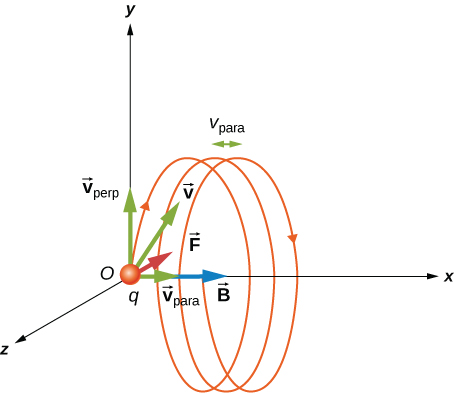
\includegraphics[width=1.1\linewidth]{figs/gyro-orbit.jpg} \\
        \tiny From phys.libretexts.org.
    \end{minipage}
\end{frame}

\begin{frame}{\gke: a computational plasma physics framework}
  %\begin{block}{Example block}
    % include simulation images
    %\vspace{.5cm}
    \begin{itemize}
        \item Continuum gyrokinetic code (3X2V) for open field lines with conducting-sheath boundary conditions
        \item Simulations: LAPD\footnote{\scriptsize Shi \etal, \emph{J. Plasma Phys.} 83.3 (2017).} (with limiter biasing), Helical field-line geometry with NSTX-SOL parameters\footnote{\scriptsize Shi \etal, \emph{Phys.~Plasmas} 26.1 (2019).}, and {\bf Texas Helimak}\footnote{\scriptsize Bernard \etal, \emph{Phys.~Plasmas} 26:4 (2019).} (with limiter biasing)
        \item Other tools:~full Vlasov-Maxwell and multi-moment fluid solvers
        \item Uses {\bf discontinuous Galerkin (DG)} finite-element method
    \end{itemize}
    %\vspace{.5cm}
\end{frame}

\begin{frame}{Discontinuous Galkerin methods efficiently solve conservative problems}
    \begin{itemize} \footnotesize
        \item (Gyro)kinetic systems require advanced computational methods to make optimal use of high-performance computing (HPC) resources
        \item {\bf Discontinuous Galkerin} method combines benefits of finite-volume methods and classic finite-element methods
    \end{itemize}%
    \begin{minipage}{.65\linewidth}
    \begin{itemize} \footnotesize
        \item Uses discontinuous basis functions to represent the numerical solution on each cell $\Omega_j$ of the computational domain
        \vspace{-.2cm}
        \begin{equation*}
            f_{h}(x,t) = \sum_{k=1}^{K} a_k(t) \varphi_k(x), \; x \in \Omega_j,
        \end{equation*}
        \vspace{-.2cm}
        \begin{itemize} \footnotesize
        \item Local and parallelizable
        \item Easily extends to higher orders
        \item Maintains conservation properties 
        \item Preserving positivity of distribution function can be challenging
        \end{itemize}
    \end{itemize}
    \end{minipage}
    \begin{minipage}{.33\linewidth}
    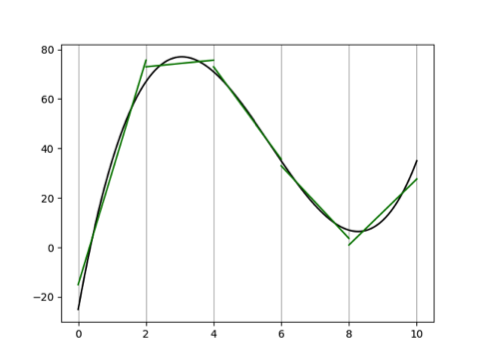
\includegraphics[width=1.1\linewidth,clip,trim=.5cm 0cm 0cm 0cm]{figs/1d-dg.png} \\
    \scriptsize DG projection of the function $(x - 5)^3 - 2x^2 + x + 100$
    \end{minipage}
\end{frame}

\section{Gyrokinetic simulations of the Texas Helimak}
\begin{frame}{Outline}
    \tableofcontents[currentsection] 
\end{frame}

\subsection{Model equations}

\begin{frame}{Electrostatic gyrokinetic model}
    \small
    \gke\ solves full-$f$ gyrokinetic system in the long-wavelength (drift-kinetic) limit, with gyrocenter distribution function $f_s(\bm{R}, v_\parallel, \mu,t)$:
    \begin{gather}
    \frac{\partial \mathcal{J}_s f_s}{\partial t} + \nabla \cdot (\mathcal{J}_s \{\bm{R},H\} f_s) + \frac{\partial}{\partial v_\parallel} (\mathcal{J}_s \{v_\parallel, H\} f_s ) =\mathcal{J}_s C[f_s] + \mathcal{J}_s S_s,     \label{eq:gk-eqn} \\
    -\nabla \cdot \left( \frac{n_{i0}^g e^2 \rho_{\mathrm{s}0}^2}{T_{e0}} \nabla_\perp \phi \right) = \sigma_g = e [n_i^g(\bm{R},t) - n_e(\bm{R},t)], \label{eq:poisson} \\
    H_s = \frac{1}{2}mv_\parallel^2 + \mu B + q_s\phi, \label{eq:ham}
    \end{gather}
    where $\mathcal{J} \approx B$, $C[f_s]$ models collisions, $S_s$ is a source term, and 
    \begin{gather*}
        \{F,G\} = \frac{\bm{B}^*}{m_s B_\parallel^*} \cdot \left( \nabla F \frac{\partial G}{\partial v_\parallel} - \frac{\partial F}{\partial v_\parallel} \nabla G \right) - \frac{1}{q_s B_\parallel^*} \bm{b} \cdot \nabla F \times \nabla G.
    \end{gather*}
    The gyrokinetic Poisson equation (\ref{eq:poisson}) uses a linearized ion guiding-center density $n_{i0}^g$ that is constant in space and time.
\end{frame}

\begin{frame}{Conducting-sheath boundary conditions}
\vspace{.5cm}
    \begin{minipage}{.62\textwidth}
        \begin{figure}
        \centering
        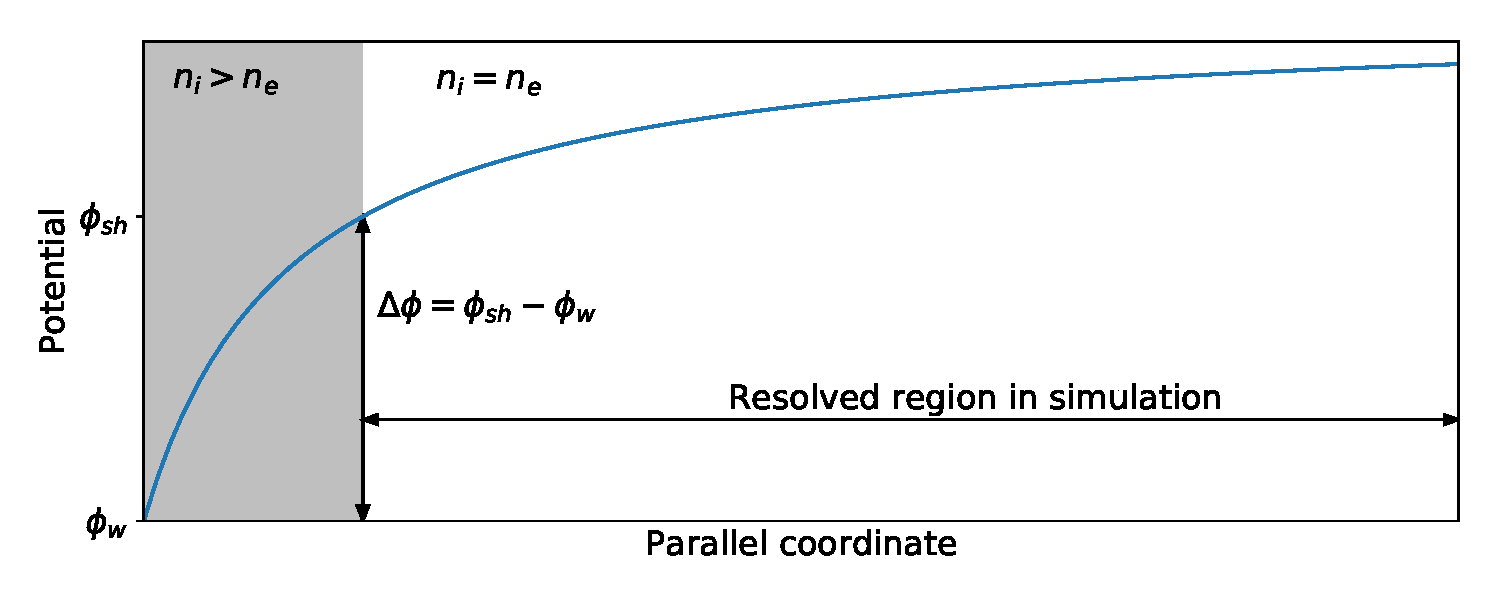
\includegraphics[width=\textwidth]{figs/cs-sw.pdf}
        \end{figure}
    \end{minipage}%
    \begin{minipage}{.35\textwidth} \scriptsize
        \begin{itemize}
            \item Allow local parallel currents into/out of sheath
            \item For now, $B \perp$ to wall%, neglecting Chodura sheaths
            \item Don't resolve the non-neutral Debye sheath 
            \item GK Poisson equation determines $\phi$ everywhere
            \item $\Delta \phi = \phi_{\rm sh} - \phi_w$
        \end{itemize}
    \end{minipage}
    \begin{minipage}{.62\textwidth}
    \vspace{.5cm}
    \begin{figure}
        \centering
        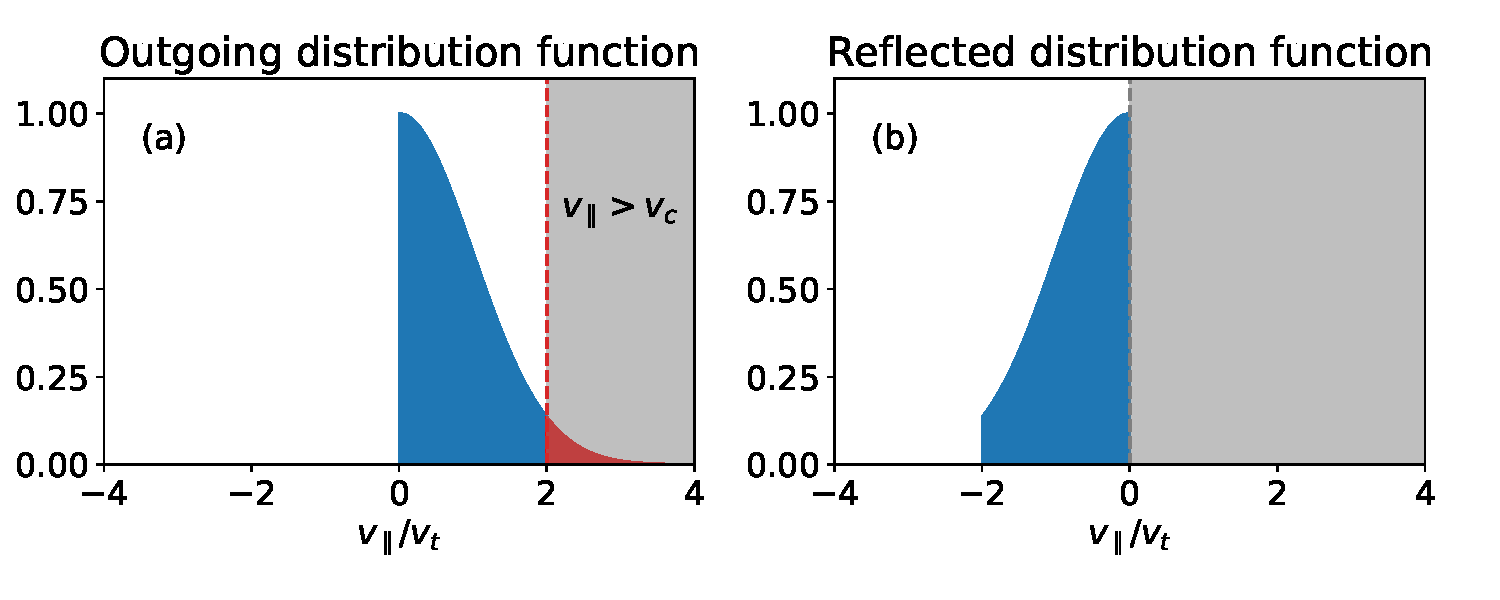
\includegraphics[width=\textwidth]{figs/dist-f-cs.pdf}
    \end{figure}
    \end{minipage}%
    \begin{minipage}{.35\textwidth} \scriptsize
        %\vspace{1cm}
        \begin{itemize}
            \item Cut-off parallel velocity for electrons given by
            $v_c = \sqrt{2e\Delta \phi/m_e}$
            \item Electrons with $\vpar > v_c$ leave the domain and with $0 < \vpar < v_c$ are reflected
            \item Free-streaming ion BCs
        \end{itemize}
    \end{minipage}%
\end{frame}

\begin{frame}{Nonorthogonal field-line following coordinates}
\vspace{.5cm}
\begin{figure}
    \centering
    % trim={<left> <lower> <right> <upper>}
    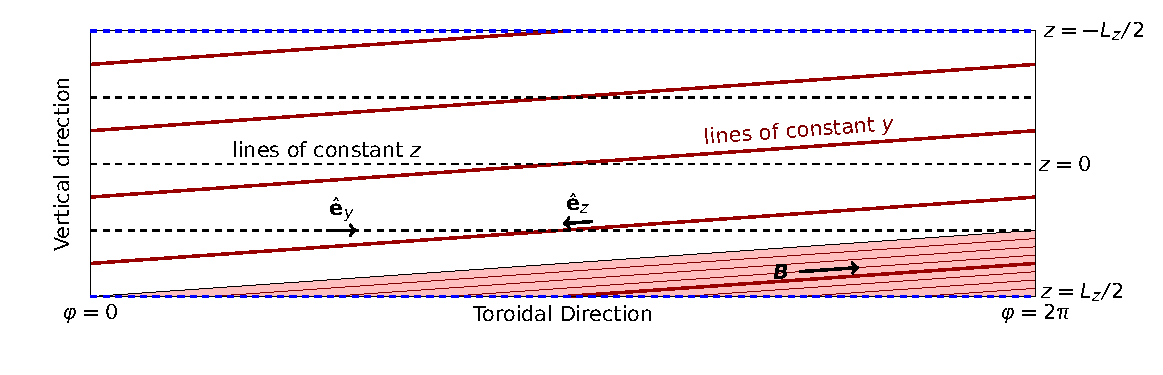
\includegraphics[trim= 0cm .5cm 0cm 1cm,width=\linewidth]{figs/helimak-B-field.pdf}
    %\caption{A map to $(r,\varphi,Z)$, shown at a slice in the radial direction for a field line with $N=4$.} % toroidal turns. Left-handed coordinate system: $(\hat{\bf{e}}_x \times \hat{\bf{e}}_y) \cdot \hat{\bf{e}}_z < 0$.}
    \label{fig:cyl-map}
\end{figure}
\vspace{-.5cm}
\begin{itemize}
\footnotesize
    \item A map to cylindrical coordinates $(r,\varphi,Z)$, shown at a slice in $R$ for a field line with $N=4$ toroidal turns.
    \item Helimak $\bm{B}$ points in the direction of decreasing $z$.
    \item Left-handed coordinate system: $(\hat{\bf{e}}_x \times \hat{\bf{e}}_y) \cdot \hat{\bf{e}}_z < 0$.
    \item $x$ is radial coordinate, $z$ is along field line and $y$ is binormal coordinate
    \item No magnetic shear
    \item BCs: Dirichlet in $x$ for $\phi$, periodic in $y$ for $f$ and $\phi$, conducting-sheath in $z$
\end{itemize}
\end{frame}

\begin{frame}{Set-up for Helimak simulations}%
\begin{minipage}{0.48\linewidth}
\footnotesize
    \centering
    \begin{tabular}{c|c}
    \textbf{Parameter} & \textbf{Value} \\ \hline
    $B_0$ & 0.1 T \\
    $n_0$ & $10^{16}$ m$^{-3}$\\
    $T_{e0}$ & 10 eV\\
    $T_{i0}$ & 1 eV\\
    $L_n$ & 0.1 m \\
    $\rho_e$ & $1.02 \times 10^{-2}$ m \\
    $\lambda_{ee}$ & 98.4 m \\
    $\rho_{\mathrm{s}0}$ & $2.04 \times 10^{-2}$ m \\
    $c_\mathrm{s}$ & $4.90 \times 10^{3}$ m/s \\
    $\lambda_{ii}$ & 1.39 m \\
    $L_x/\rho_{s0} $ & 50 \\
    $L_z$ & 40.0 m \\
    $\tau_\parallel$ & 4.08 ms 
	\end{tabular}
\end{minipage}%%
\begin{minipage}{0.48\linewidth}
\vspace{.25cm}
\begin{itemize}
\footnotesize
    \item Piecewise linear basis functions
    \item Reduced ion-to-electron mass ratio: $m_i/m_e = 400$
    \item Simulated 16 ms $\sim$4$\tau_\parallel$ 
    \item $\sim$180k CPU-hours on TACC Stampede2 SKX compute nodes
\end{itemize}
\end{minipage}
\end{frame}

\begin{frame}{1D fluid model approximates Helimak source}
    \footnotesize
    \begin{itemize}
        \item Electrons are preferentially heated by electron-cyclotron and upper-hybrid resonances. $\sim90\%$ lost to radiation.
        \item Power deposition not accurately known. 
        \item Use Gaussian source of the form:
    \end{itemize}%
    \begin{equation}
    \label{eq:source-profile}
    S_s(\bm{R}, v_\parallel, \mu) = S_0 \exp[-(x - x_\mathrm{src})^2 / (2\sigma_\mathrm{src}^2)] F_M(v_\parallel, \mu; T_{s,\mathrm{src}}),
    \end{equation}%
    \vspace{-.25cm}
    \begin{itemize}
        \item Balance source rate to end-plate losses, assuming a steady-state density profile based on 1D fluid model\footnote{\scriptsize Shi, \emph{et al., Phys.~Plasmas} 26.1 (2019).}:
    \end{itemize}%
    \begin{equation}
    \label{eq:dens-source}
    n(x,z) = n_{p} \exp \left [-(x - x_\mathrm{src})^2 / \left (2\sigma_n^2 \right ) \right ] \frac{1 +\sqrt{1 - z^2/(L_z/2)^2}}{2}
    \end{equation}%
    \vspace{-.25cm}
        \begin{itemize}
        \item Using $x_\mathrm{src}=1.0$ m, $\sigma_\mathrm{src}=0.01$ and Eqns.~(\ref{eq:source-profile}) and (\ref{eq:dens-source}) gives: $S_0 \approx 9.77 \times 10^{19}$ m$^{-3}$s$^{-1}$, $T_{i,{\rm src}}=\frac{5}{3}T_{i0}$, $T_{e,{\rm src}}=\frac{10}{3}T_{e0}$
        \item Radiation and neutral-interactions only modeled \emph{indirectly} through net source rate.
    \end{itemize}
\end{frame}

\begin{frame}{Simulations reproduce interchange-like turbulence}
\begin{figure}
    \centering
    \includemedia[
    activate=pageopen,
    width=\linewidth,
    height=.2\linewidth,
    keepaspectratio,
    addresource=figs/figure6-movie.mp4,
    flashvars={source=figs/figure6-movie.mp4
    &autoPlay=true%    % optional configuration
    &loop=true%        % variables
    }  
    ]{}{VPlayer.swf}
    %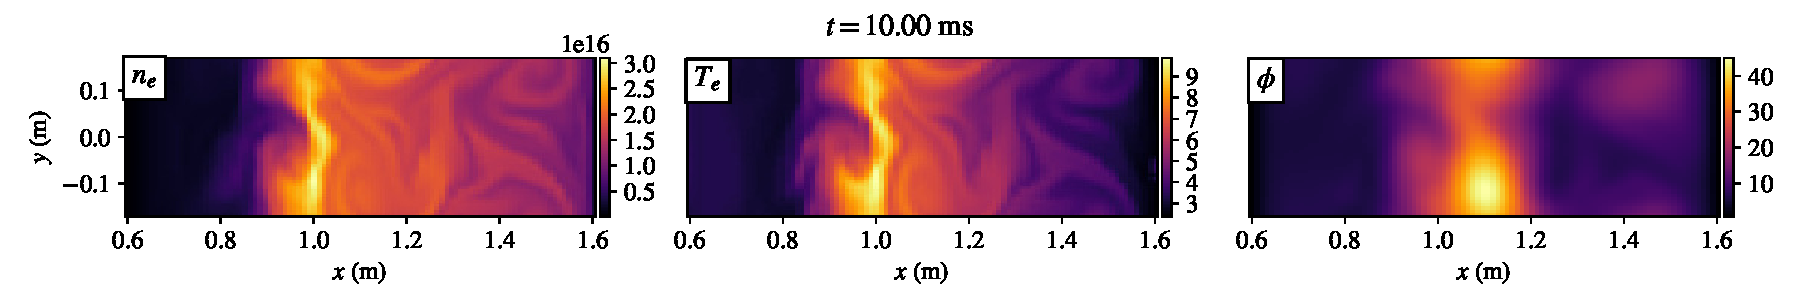
\includegraphics[width=\linewidth]{figs/figure6-eps-converted-to.pdf}
    \caption{From left to right, electron density (m$^{-3}$), electron temperature (eV), and electrostatic potential (V) in ($x,y$) in the field-line-following coordinate system at the midpoint in $z$ shown from 10--16 ms.}
\end{figure}%
\begin{figure}
    \begin{minipage}{0.6\linewidth}
    \centering
    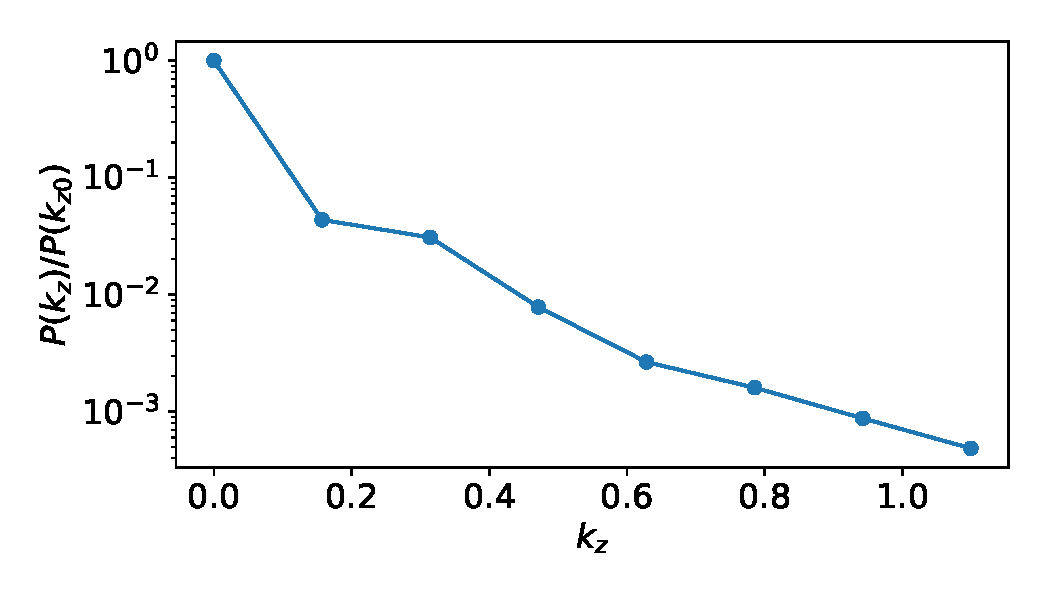
\includegraphics[width=.9\linewidth]{figs/kz-line.pdf}
    \end{minipage}%
    \begin{minipage}{0.4\linewidth}
    \caption{Power in the Fourier transform in $z$ of electron density fluctuations, averaged in $x$ and $y$ and from 10 to 16 ms. The power in the zeroth mode is at least ten times greater than the other modes, suggesting average $k_z \approx 0$.}
    \label{fig:my_label}
    \end{minipage}
\end{figure}
\end{frame}

\begin{frame}{Simulation mapped to cylindrical coordinates}
\begin{minipage}{\linewidth}
\begin{figure}
    \centering
    \includemedia[
    activate=pageopen,
    width=\linewidth,
    height=.4\linewidth,
    keepaspectratio,
    addresource=figs/figure7-movie.mp4,
    flashvars={source=figs/figure7-movie.mp4
    &autoPlay=true%    % optional configuration
    &loop=true%        % variables
    }  
    ]{}{VPlayer.swf}
    %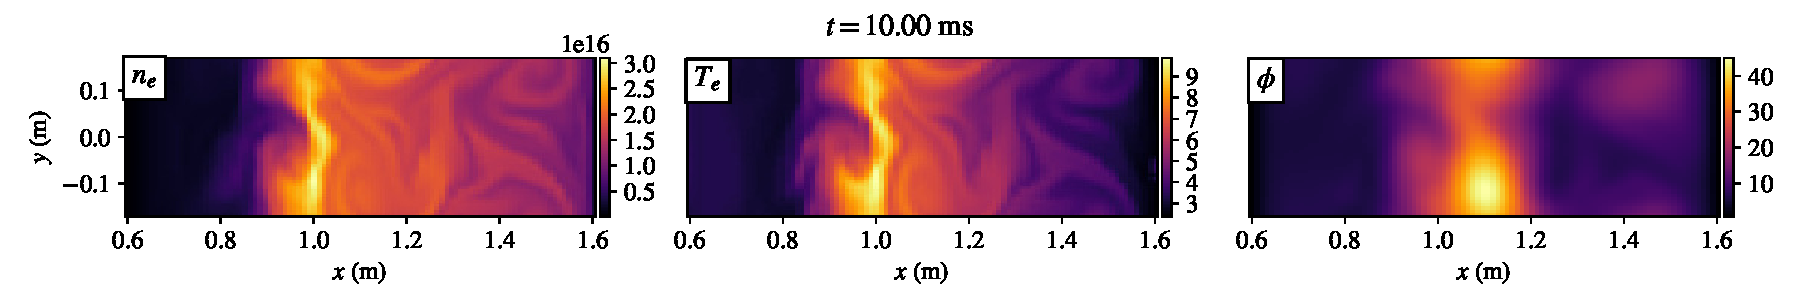
\includegraphics[width=\linewidth]{figs/figure6-eps-converted-to.pdf}
    \caption{From left to right, electron density (m$^{-3}$), electron temperature (eV), and electrostatic potential (V) in ($R,Z$) in cylidrical coordinates at a slice in $\varphi$ from 10 to 16 ms using the transformation below.}
\end{figure}%
\end{minipage} \footnotesize
\begin{eqnarray}
    \label{eq:flux-map1}
    Z &=& -2.0z/L_z + 1.0  \\ 
    \label{eq:flux-map2}
    \varphi &=& \frac{2\pi}{L_y}\left(y + \frac{2.0z}{L_z} - 1.0\right)
\end{eqnarray}
\end{frame}

\subsection{Validation with experimental data}
\begin{frame}{Simulation captures features of experimental equilibrium profiles}
\begin{minipage}{.5\linewidth}
\begin{figure}
    \centering
    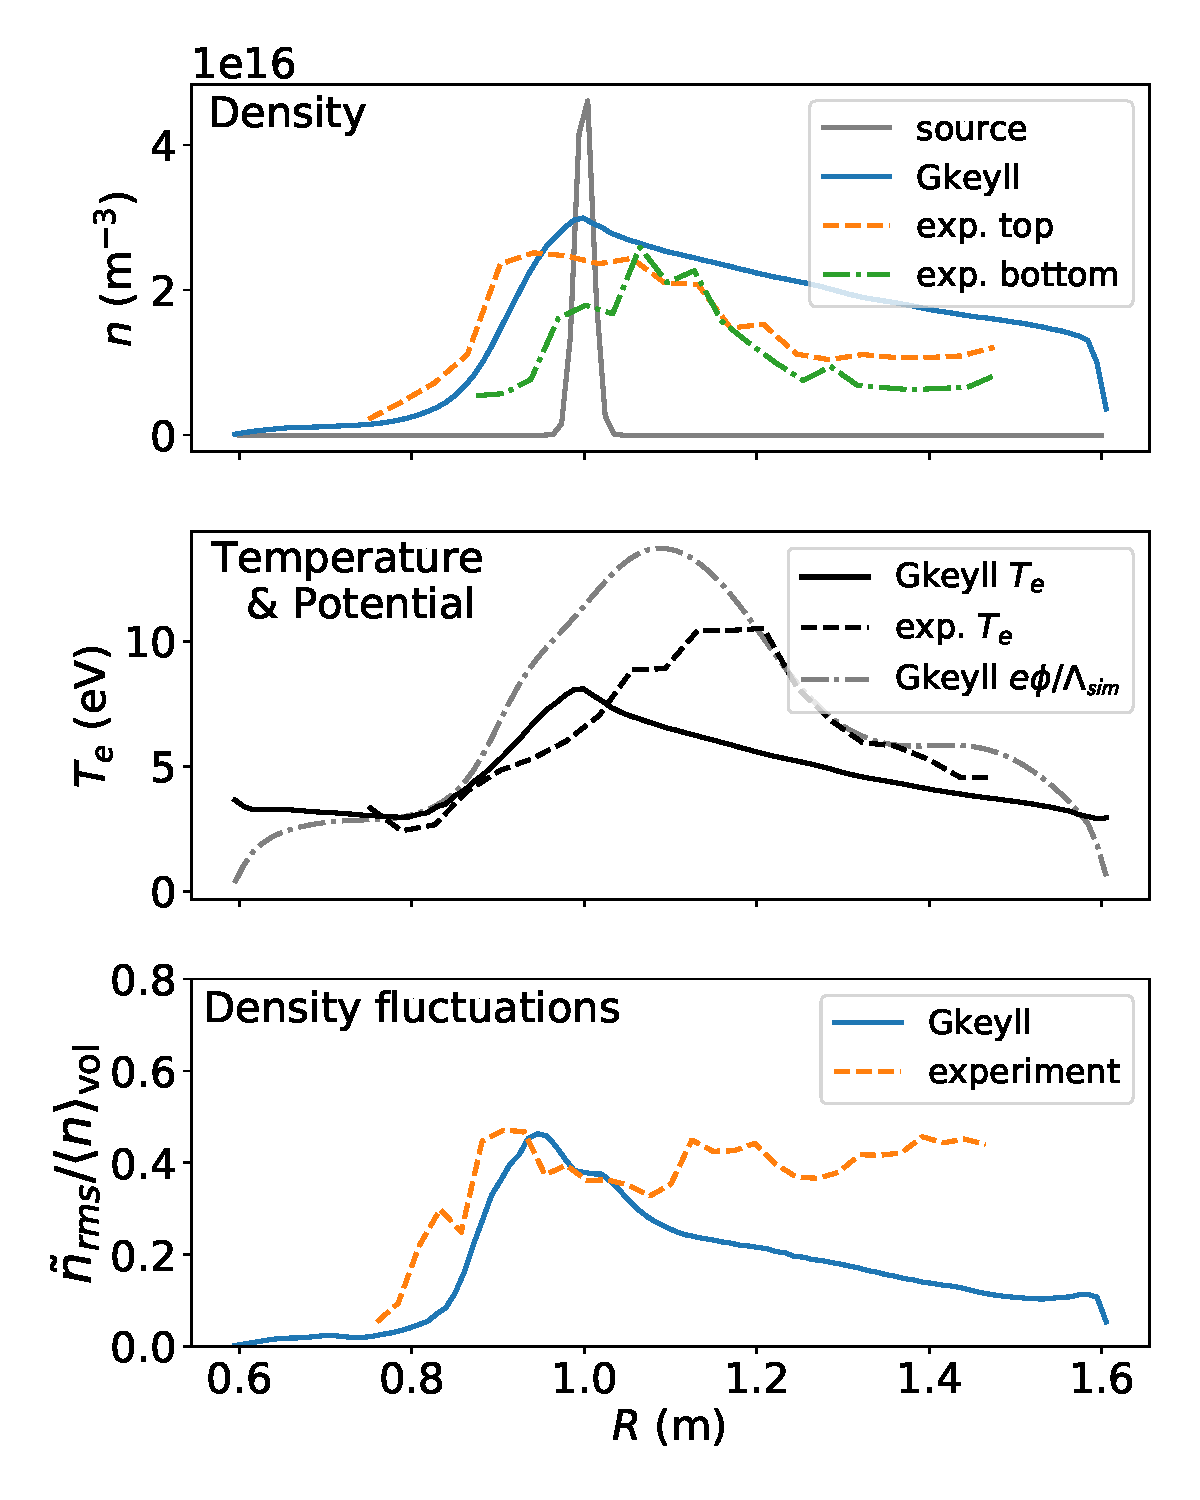
\includegraphics[width=\linewidth]{figs/eqprof-sw.pdf}
    %\caption{Caption}
    \label{fig:my_label}
\end{figure}
\end{minipage}%
\begin{minipage}{.5\linewidth}
\begin{itemize}
\scriptsize
    \vspace{-1cm}
    %\item Narrow source (in gray) broadened by turbulence.
    \item Simulation reproduces density magnitude and gradients relatively well.
    \item Top-bottom asymmetry in experiment not captured: simulations currently do not have vertical $E\times B$ flow.
    \vspace{.7cm}
    \item Slightly underpredicts $T_e$ magnitude and gradient at high $R$.
    \vspace{1cm}
    \item Density fluctuation levels approach experimental values much better than previous fluid simulations.
    \item Deviations at high $R$ could improve with full non-linear Poisson equation.
\end{itemize}
\end{minipage}

\end{frame}

\begin{frame}{Vertical $E \times B$ flow may be important}
\vspace{.5cm}
\begin{figure}
    \centering
    % trim={<left> <lower> <right> <upper>}
    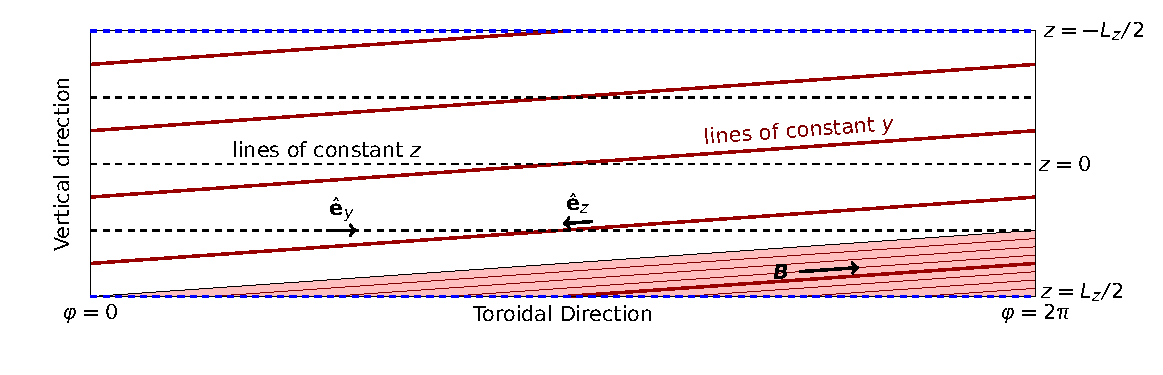
\includegraphics[trim= 0cm .5cm 0cm 1cm,width=\linewidth]{figs/helimak-B-field.pdf}
    %\caption{A map to $(r,\varphi,Z)$, shown at a slice in the radial direction for a field line with $N=4$.} % toroidal turns. Left-handed coordinate system: $(\hat{\bf{e}}_x \times \hat{\bf{e}}_y) \cdot \hat{\bf{e}}_z < 0$.}
    \label{fig:cyl-map}
\end{figure}
% \begin{itemize}
%\footnotesize
%     \item A map to $(r,\varphi,Z)$, shown at a slice in the radial direction for a field line with $N=4$ toroidal turns.
%     %\item Helimak $\bm{B}$ points in the direction of decreasing $z$. 
%     \item Left-handed coordinate system: $(\hat{\bf{e}}_x \times \hat{\bf{e}}_y) \cdot \hat{\bf{e}}_z < 0$.
% \end{itemize}
\vspace{-.5cm}
\footnotesize
Advection due to radial $\bm{E}$ and parallel flow:
\begin{align}
    V_E \cdot \nabla + V_\parallel \frac{\partial}{\partial z} &= 
    \left( V_E \cdot \nabla y \right) \frac{\partial}{ \partial y} + \left( V_E \cdot \nabla z \right) \frac{\partial}{ \partial z} + V_\parallel \frac{\partial}{\partial z} \\
    &\cong |V_E| \left( \frac{\partial}{ \partial y} - \cancel{\frac{B_\varphi}{B_Z} \frac{\partial}{\partial z}}\right) + V_\parallel \frac{\partial}{\partial z} 
\end{align}
Like most core flux-tube codes, we neglect the second term, assuming $k_{\perp} \gg k_{||}$. This term has little direct effect on turbulence, but can cause up-down asymmetries in equilibrium profiles when $B_\varphi/B_Z$ is large.
\end{frame}

\begin{frame}{Turbulence statistics compared at max($V_E$)}
    %Edit images here
\begin{minipage}{.5\linewidth}
\begin{figure}
    \centering
    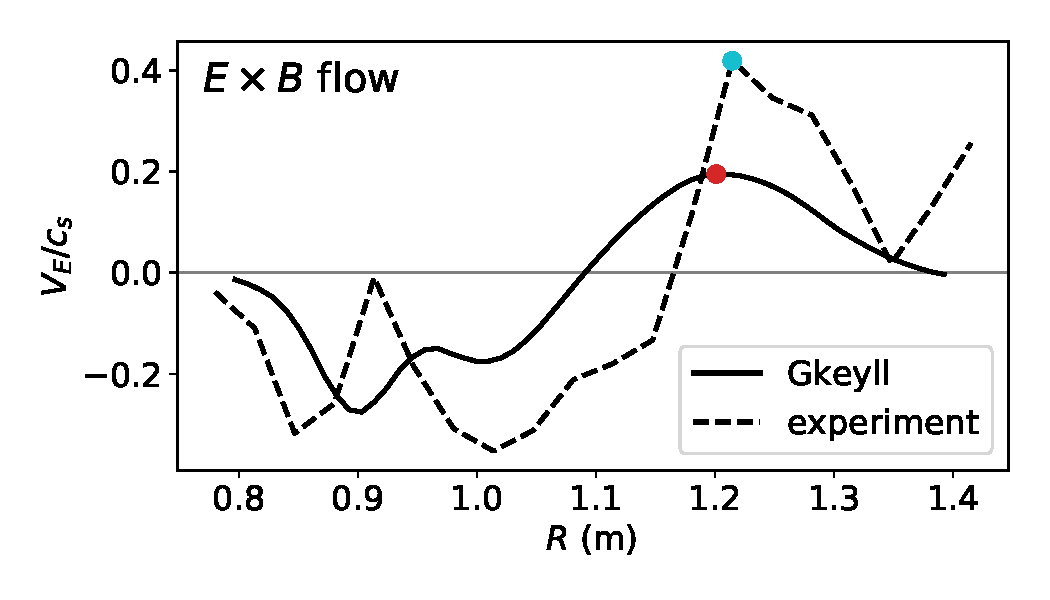
\includegraphics[width=.8\linewidth]{figs/ve-sw.pdf} \\
    \vspace{-.2cm}
    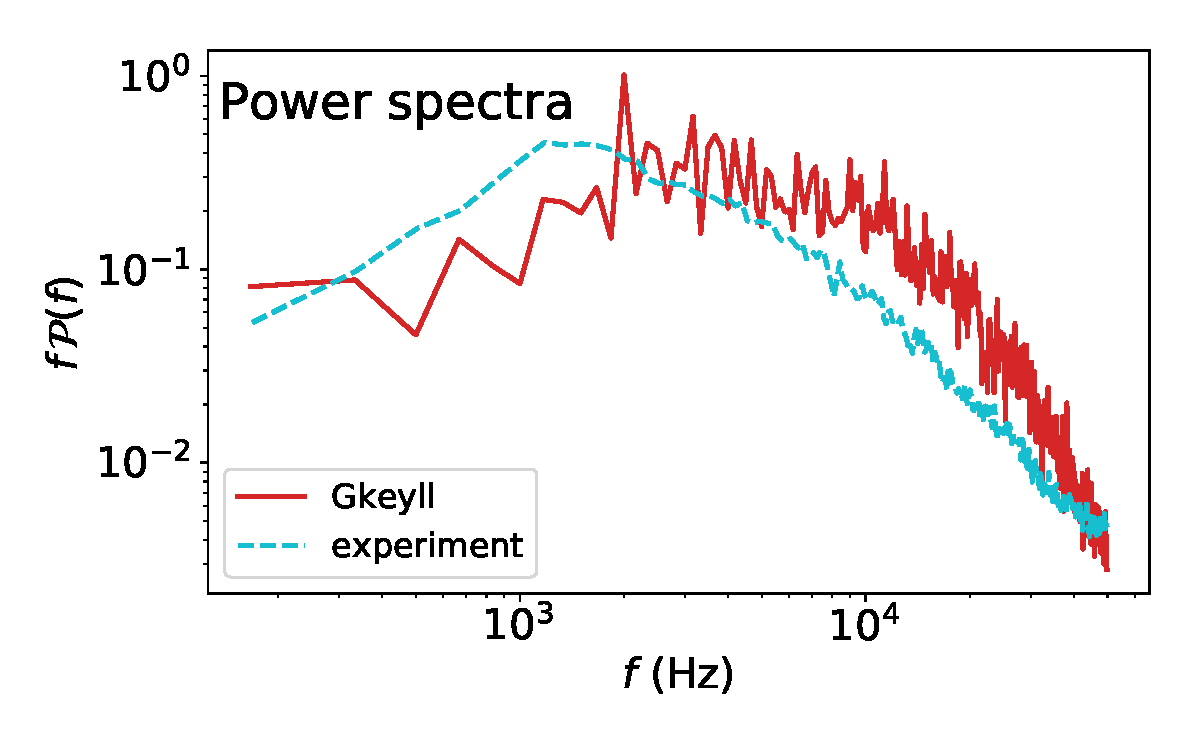
\includegraphics[width=.8\linewidth]{figs/fft-ttf.pdf} \\ \vspace{-.2cm}
    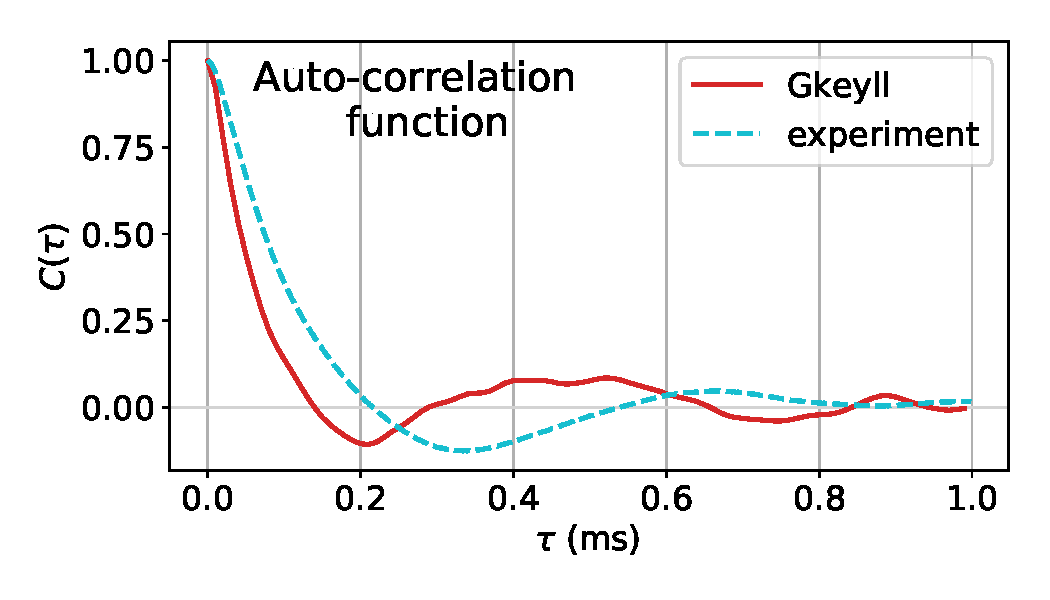
\includegraphics[width=.8\linewidth]{figs/autocorr-sw.pdf}
    %\caption{Caption}
    \label{fig:ve-shear}
\end{figure}
\end{minipage}%
\begin{minipage}{.5\linewidth}
\scriptsize
\begin{itemize}
    \vspace{-1cm}
    \item $V_E = -(d\phi_0/dx)/B_0$. 
    \item Experimental $V_E$ calculated from $T_e$ profiles, assuming adiabatic electrons.
    % \vspace{1cm}
    % \item Shear $\gamma_E = |dV_E/ dx|$ compared to local linear interchange growth rate $\gamma_I = c_s/\sqrt{R L_p}$
    \vspace{1.5cm}
    \item Power spectra of density fluctuations normalized to total energy: \\
    $\mathcal{P}(f) = \frac{\langle |\tilde{n}(f)|^2 \rangle}{\sum_f \Delta f |\tilde{n}(f)|^2}$
    \item Simulation is noisier, peaks at a higher frequency, and decays more quickly.
    \vspace{1cm}
    \item $C(\tau) = \langle \tilde{n}(t) \tilde{n}(t+\tau) \rangle / \langle \tilde{n}(t)^2 \rangle$
    \item Correlation time for the simulation data is shorter.
\end{itemize}
\end{minipage}
\end{frame}

\begin{frame}{Simulation captures turbulence intermittency}
\begin{minipage}{.5\linewidth}
\begin{figure}
    \vspace{.5cm}
    \centering
    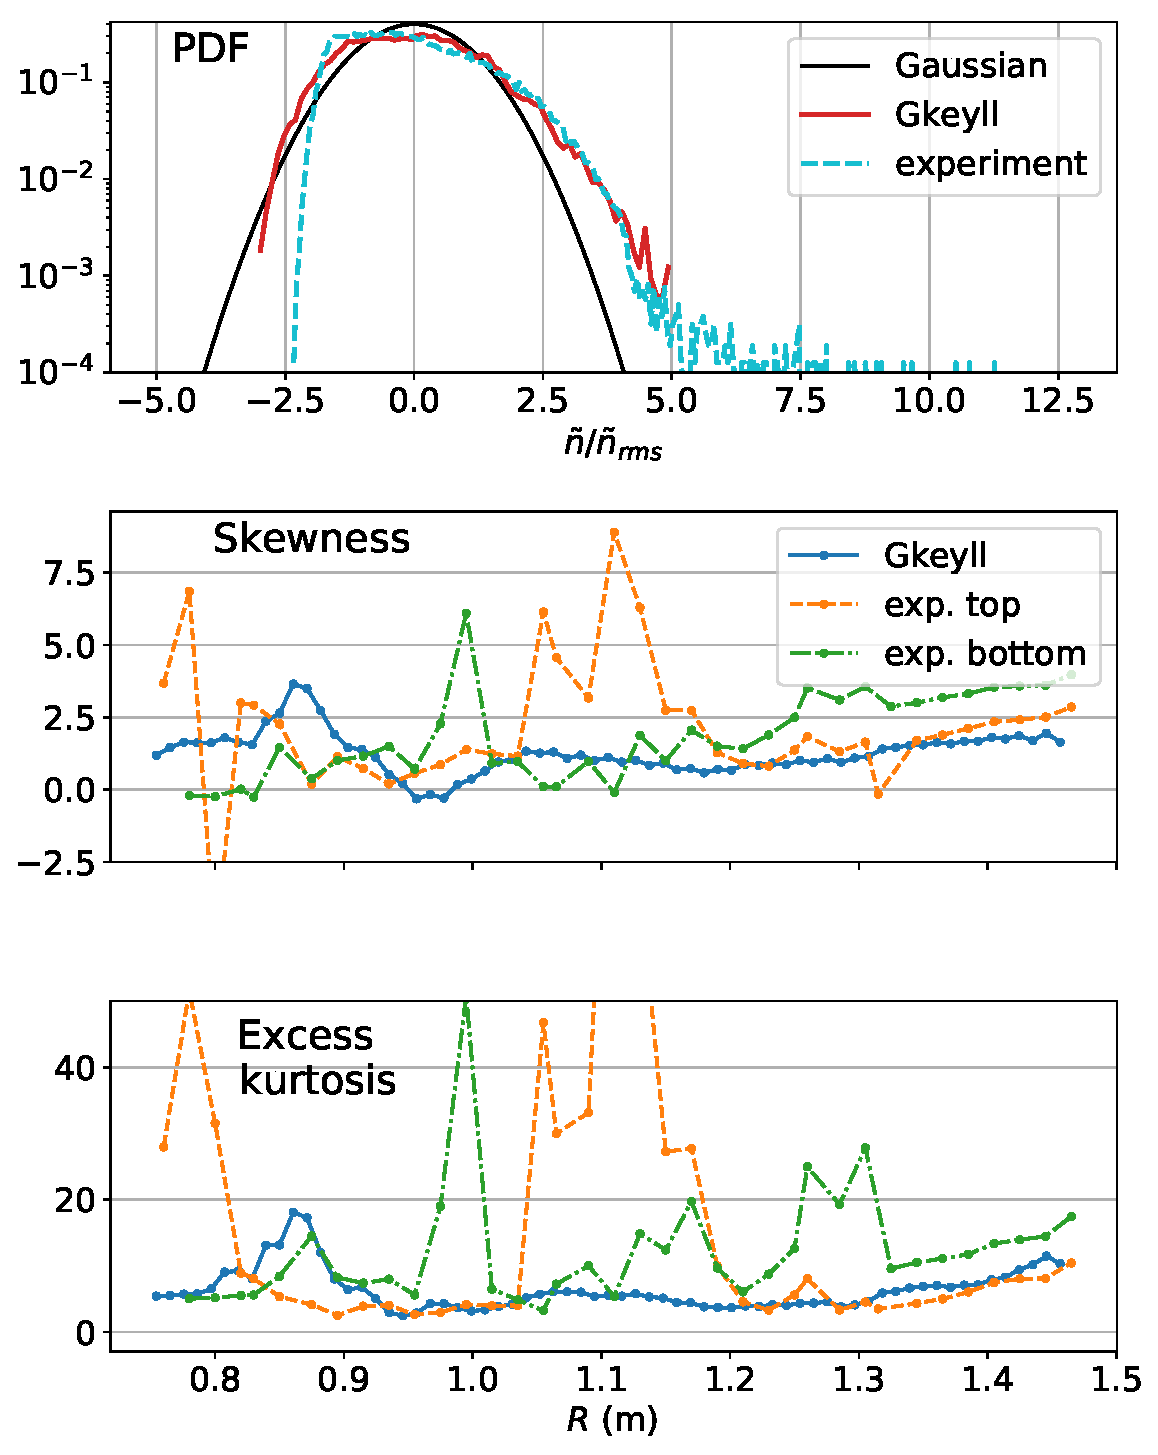
\includegraphics[width=\linewidth]{figs/pdf-skew-kurt-sw.pdf}
    \label{fig:my_label}
\end{figure}%
\end{minipage}%
\begin{minipage}{.5\linewidth}
% \begin{figure}
%     \centering
%     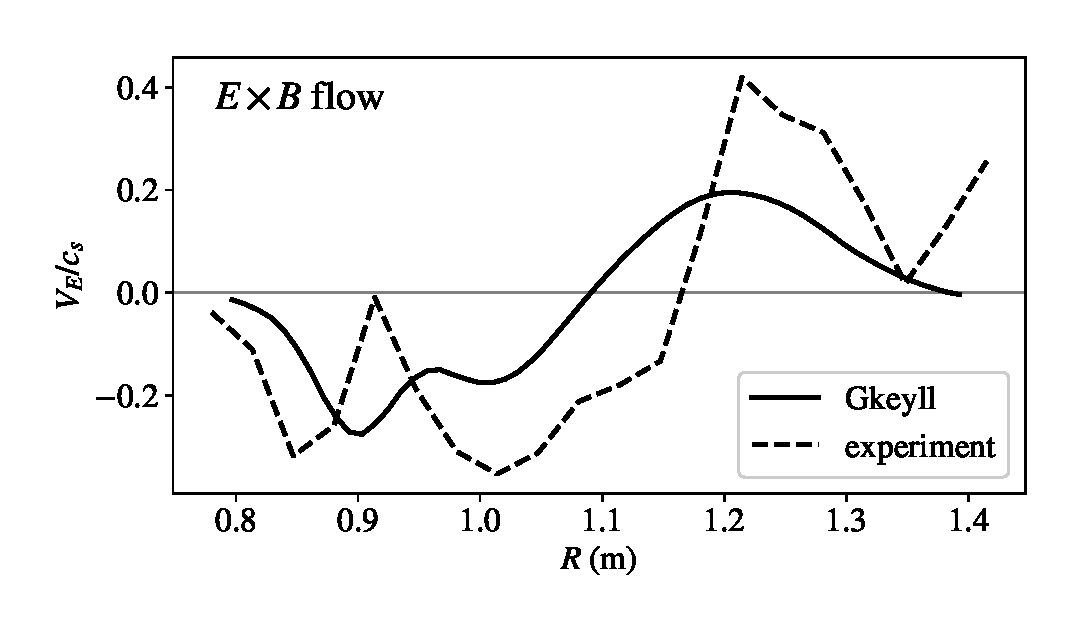
\includegraphics[width=.8\linewidth]{figs/ve-ttf.eps}
%     \label{fig:my_label}
% \end{figure}
\begin{itemize}
\footnotesize
\vspace{-.5cm}
    \item Positive tails of the simulation PDF's approach the experimental values until $5\tilde{n}/n_{\rm rms}$. 
    \item Longer simulations could attain longer experimental tails.
    \vspace{1.5cm}
    \item Skewness = $E[\tilde{n}^3]/\sigma^3$
    \item Excess kurtosis  =$E[\tilde{n}^4]/\sigma^4 - 3$
    \item Positive skewness and excess kurtosis signal intermittent turbulence, a sign of blob transport.
    %\item $E[...]$ is the expectation value and $\sigma$ is standard deviation
\end{itemize}
\end{minipage}%
\end{frame}

\begin{frame}{Kinetic effects are relatively small}
    \begin{minipage}{.5\linewidth}
    \vspace{.5cm}
        \begin{figure}
            \centering
            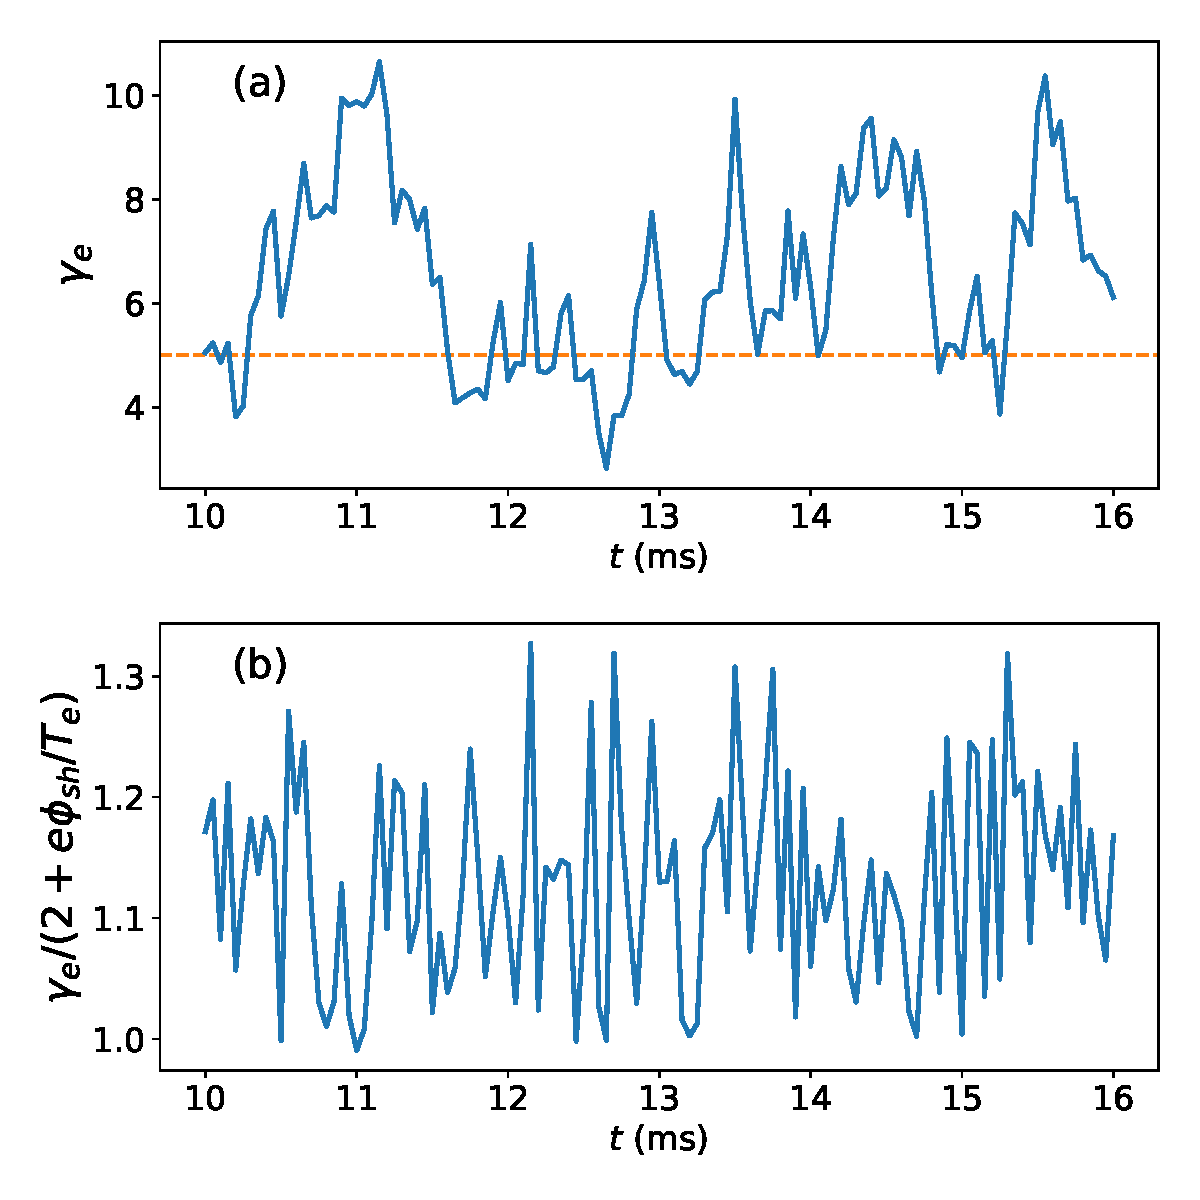
\includegraphics[width=\linewidth]{figs/heat-coef-sw.pdf}
            \caption{Time evolution of electron sheath heat-transmission coefficient}
            \label{fig:my_label}
        \end{figure}
    \end{minipage}%
    \begin{minipage}{.5\linewidth}
    \begin{itemize} \footnotesize
        \item (a) $\gamma_e = q_\parallel/(\Gamma_{\parallel,n} T_e)$, with quantities evaluated at the sheath entrance, $z=L_z/2$, and at the midpoint in $y$
        \item (b) $\gamma_e$ normalized to the expected value for a Maxwellian distribution function, $2 + e\phi_{\rm sh}/T_e$
        \item $\gamma_e$ fluctuates in time and exceeds expected Maxwellian value by approximately 10--20\%.
        \item Indicates relatively small kinetic effects.
    \end{itemize}
    \end{minipage}
\end{frame}

\begin{frame}{Additional features could improve comparison}
    \begin{itemize}
        \item Vertical $E \times B$ flow: transport and equilibrium profiles
        \item Magnetic shear: turbulence statistics
        \item Real electron mass: turbulence levels (by increasing response of electrostatic potential to temperature fluctuations at sheath)
        \item Full non-linear Poisson equation
        \item Other considerations: radiation, neutral model, improved sheath BCs
    \end{itemize}
\end{frame}

\subsection{Limiter-biasing simulations}
\begin{frame}{Shear flow can reduce plasma turbulence levels}
\vspace{.5cm}
\begin{minipage}{.4\linewidth}
\centering
Turbulent eddies in the \\ presence of velocity shear...
\end{minipage}
\hfill
\begin{minipage}{.5\linewidth}
\centering
...can become stretched and \\ eventually break apart.
\end{minipage}
    \begin{figure}
        \centering
        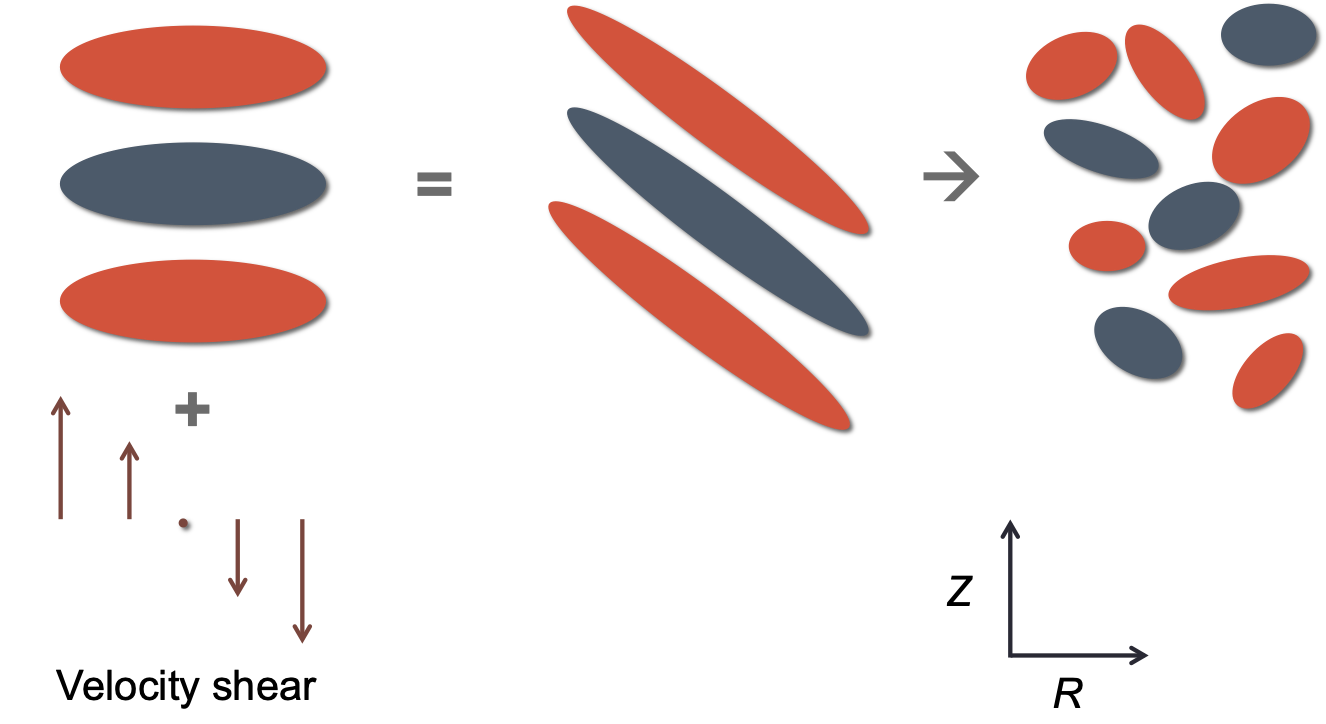
\includegraphics[width=.9\linewidth]{figs/shear-cartoon.png}
    \end{figure}
\end{frame}

\begin{frame}{Limiter biasing modifies shear flow in SMTs}
\begin{minipage}{.45\linewidth}
    \begin{itemize}\footnotesize
        \item Velocity shear in strongly magnetized plasmas can have stabilizing effect by breaking apart turbulent eddies
        \item Potentially important for understanding L-H transition
        \item Requirements for stabilization of turbulence by shear:
        \begin{enumerate}\scriptsize
            \item Shear rate is greater than the turbulence decorrelation rate
            \item Turbulent structures remain in the region of shear longer than the decorrelation time
            \item Flow is stable, i.e.~not Kelvin-Helmholtz unstable
        \end{enumerate}
    \end{itemize}
\end{minipage}%
\hfill
\begin{minipage}{.5\linewidth}
\begin{figure}
    \centering
    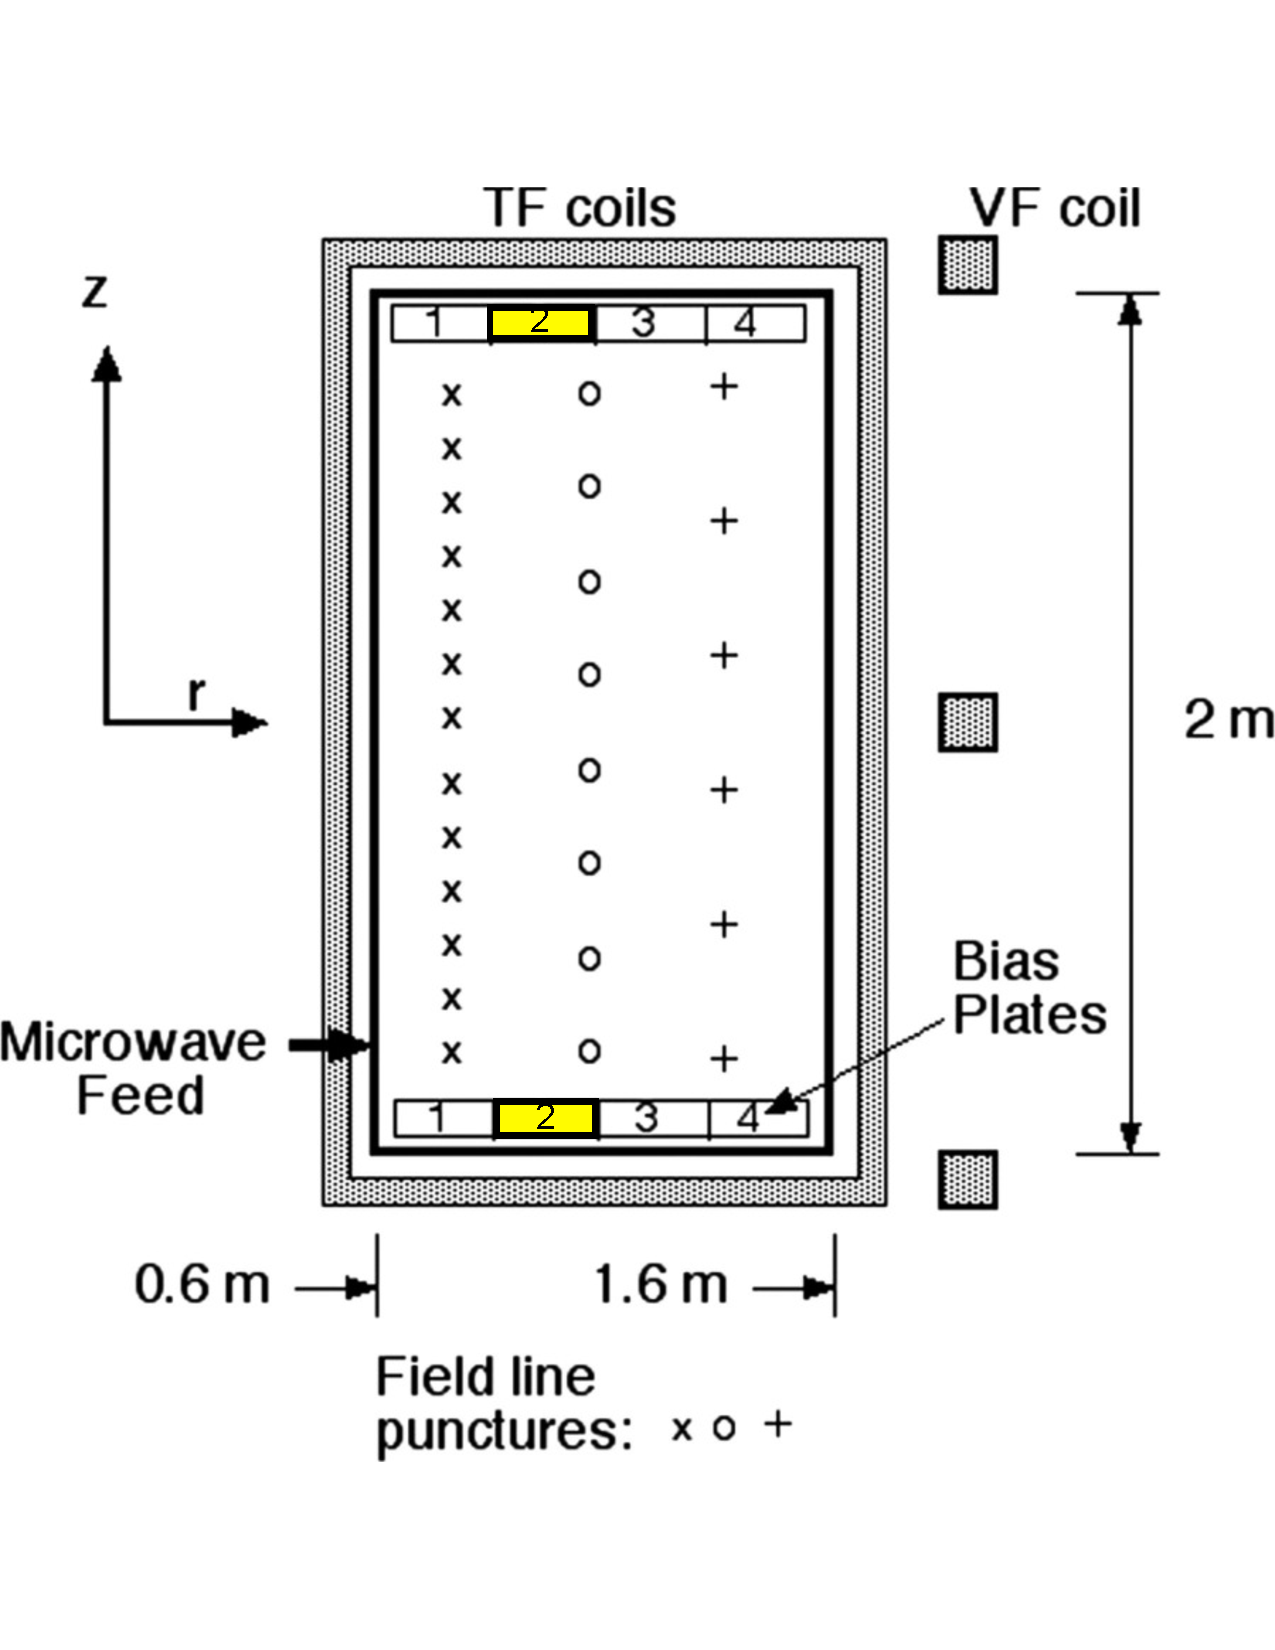
\includegraphics[width=.7\linewidth]{figs/figure1.pdf}
    \label{fig:my_label}
\end{figure}
\vspace{-.5cm}
\begin{itemize} \footnotesize
\item \gke\ models biasing via conducting-sheath BCs in $z$:
\end{itemize}
\footnotesize
    \begin{equation*}
    \label{eq:bc-bias}
    \phi_\mathrm{w}(x,y) = 
    \begin{cases} 
      V_b & 0.86 \leq x \leq 1.06 \\
      0 & \mathrm{else}
    \end{cases}
    \end{equation*}
\end{minipage}
\end{frame}

\begin{frame}{Small effect on simulation equilibrium profiles}
    \begin{figure}
        \centering
        Simulation
        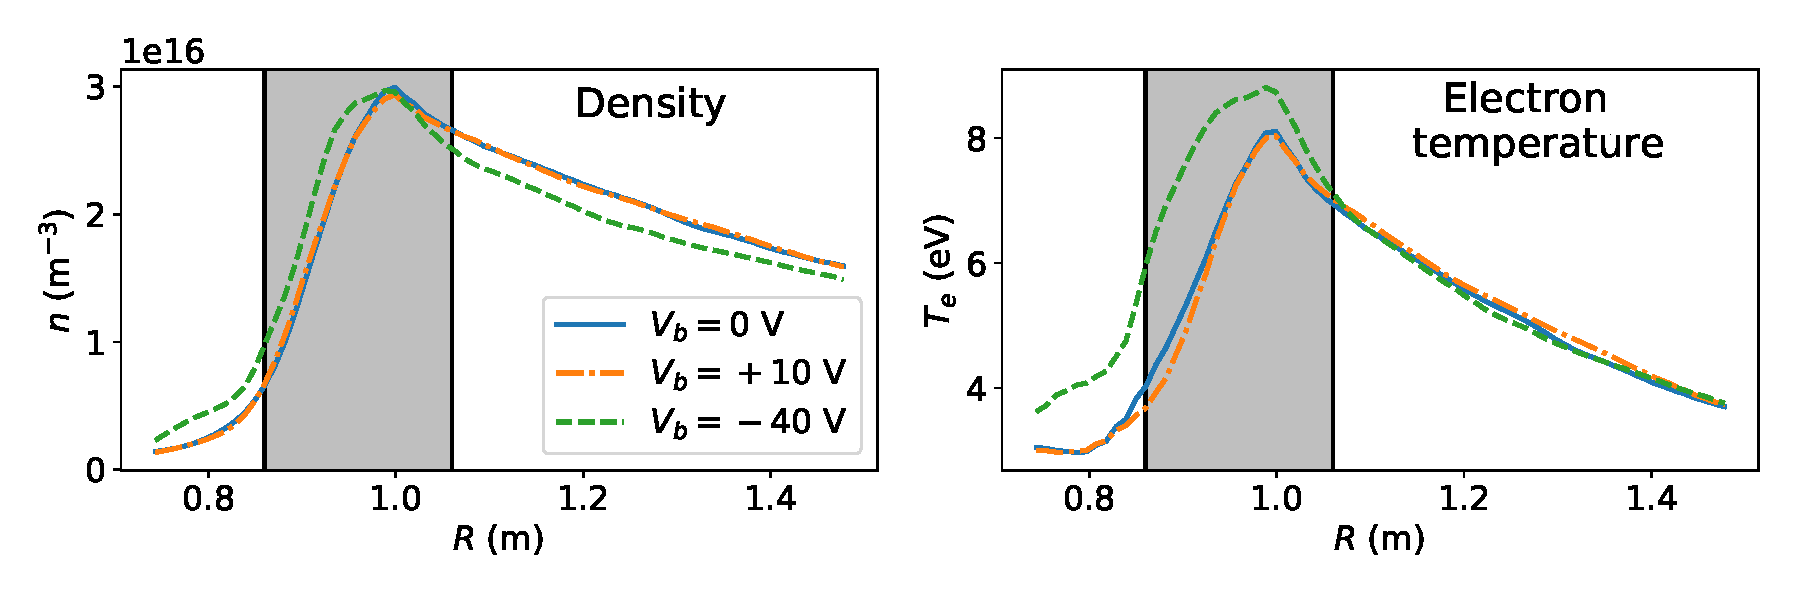
\includegraphics[width=.9\textwidth]{figs/nT-bias-sw.pdf}
        %\caption{Caption}
        \label{fig:my_label}
    \end{figure}
    \vspace{-.5cm}
    \begin{figure}
        \centering
        Experiment
        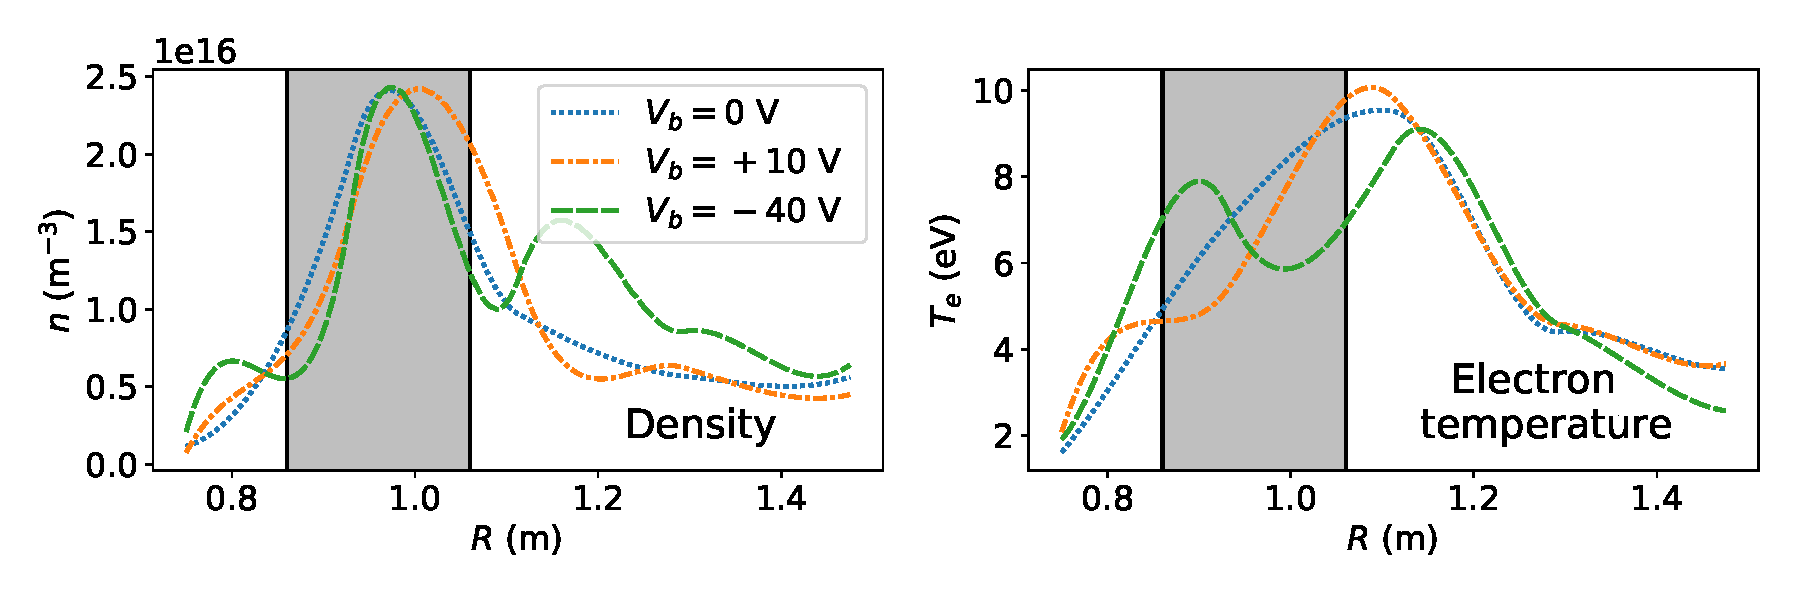
\includegraphics[width=.9\textwidth]{figs/nt-exp-sw.pdf}
        %\caption{Caption}
        \label{fig:my_label}
    \end{figure}
\end{frame}

\begin{frame}{Compare shear to local linear growth rate \small $\gamma_I = c_s/\sqrt{RL_p}$}
\vspace{-.5cm}
    \begin{figure}
        \centering
        Simulation
        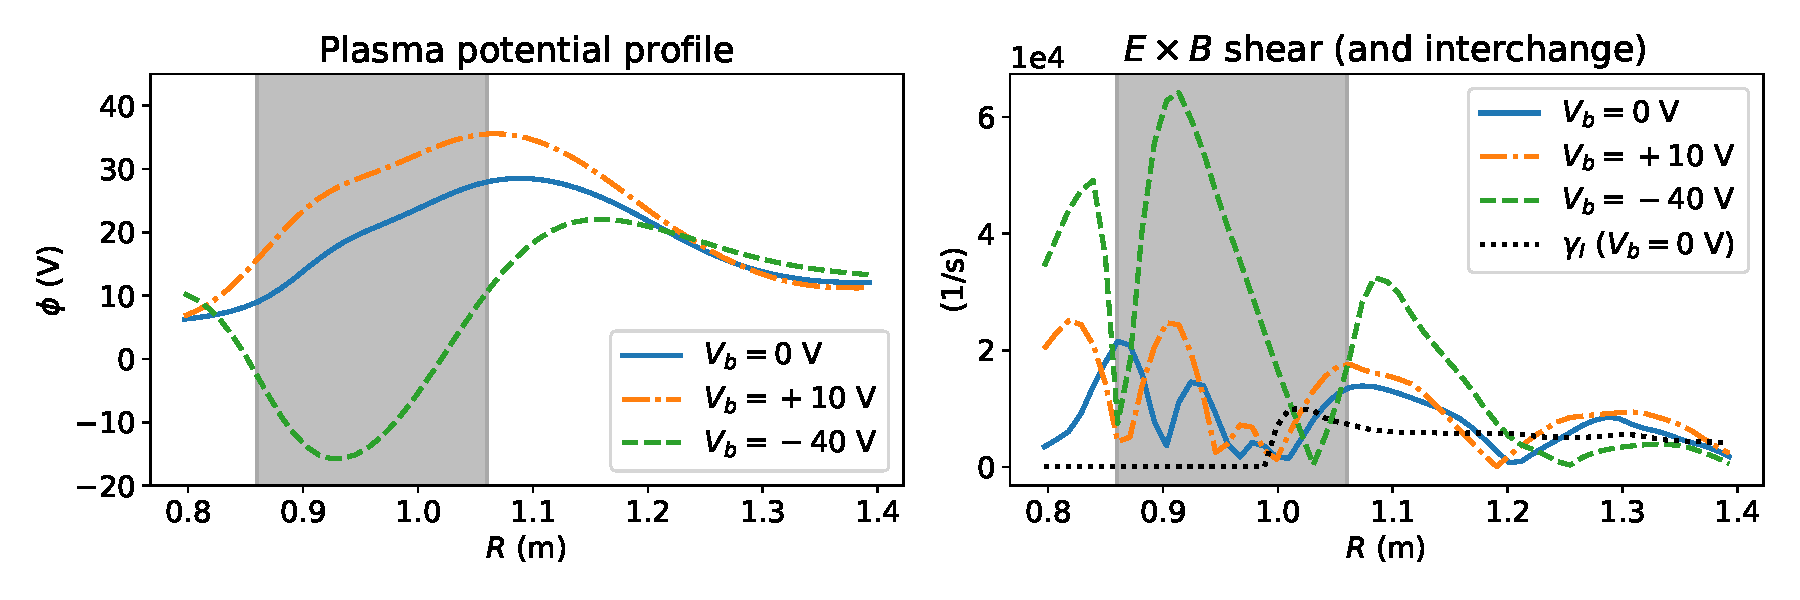
\includegraphics[width=.9\textwidth]{figs/phi-gamma-sim.pdf}
        %\caption{Caption}
        \label{fig:my_label}
    \end{figure}
    \vspace{-.75cm}
    \begin{figure}
        \centering
        Experiment
        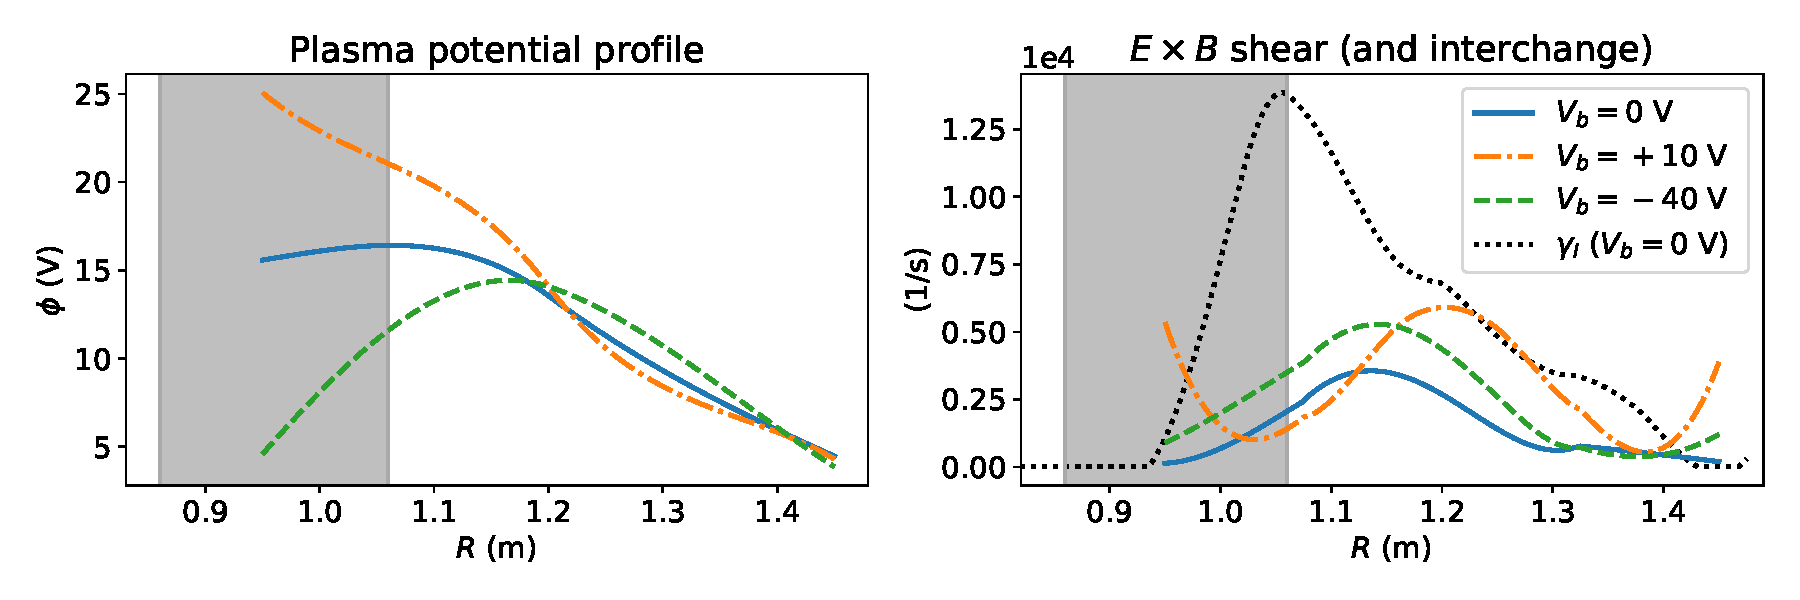
\includegraphics[width=.9\textwidth]{figs/phi-gamma-exp.pdf}
        %\caption{Caption}
        \label{fig:my_label}
    \end{figure}
\end{frame}

\begin{frame}{Turbulence levels correlate with linear growth rates \small $\gamma_I = c_s/\sqrt{RL_p}$}
\vspace{-.5cm}
    \begin{figure}
        Simulation \\
        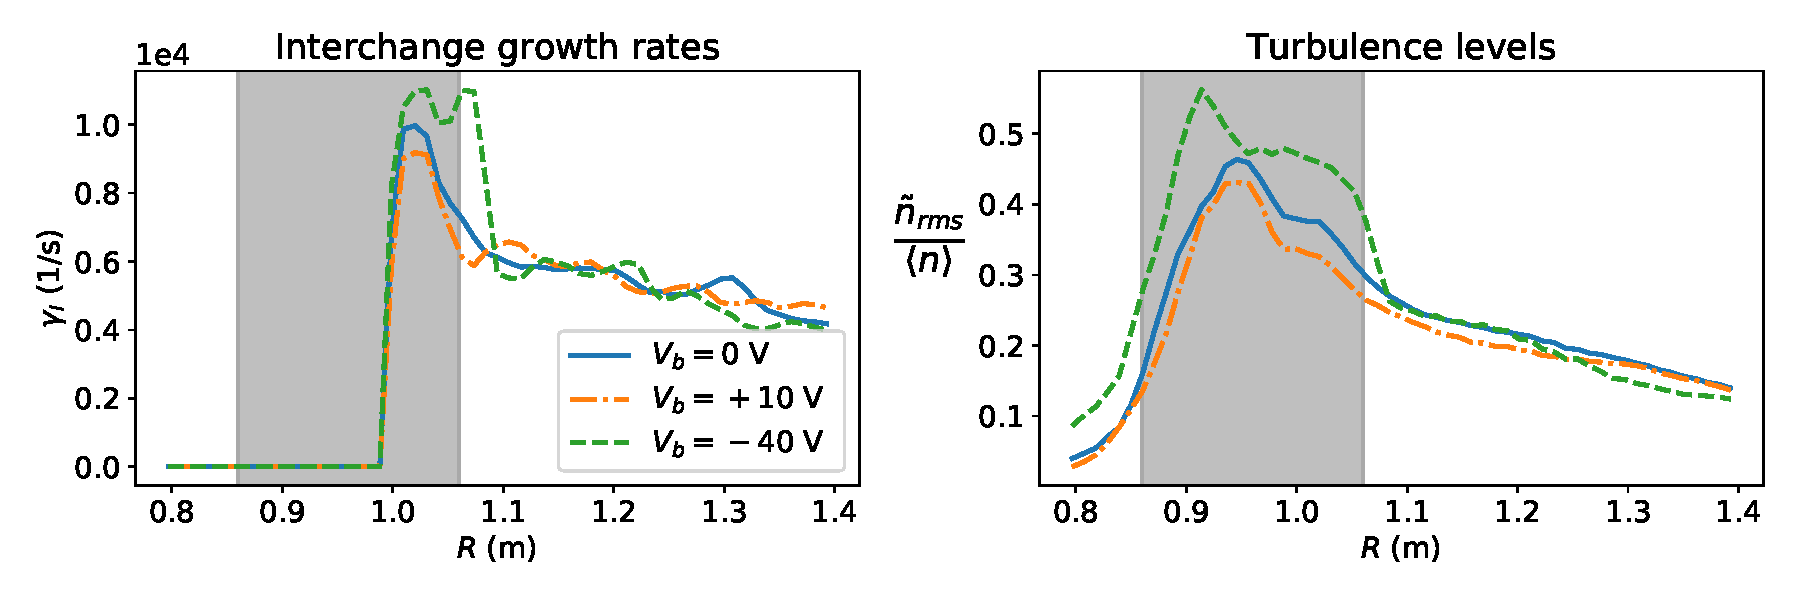
\includegraphics[width=.9\linewidth,left]{figs/gamma-dn-sim.pdf}
        %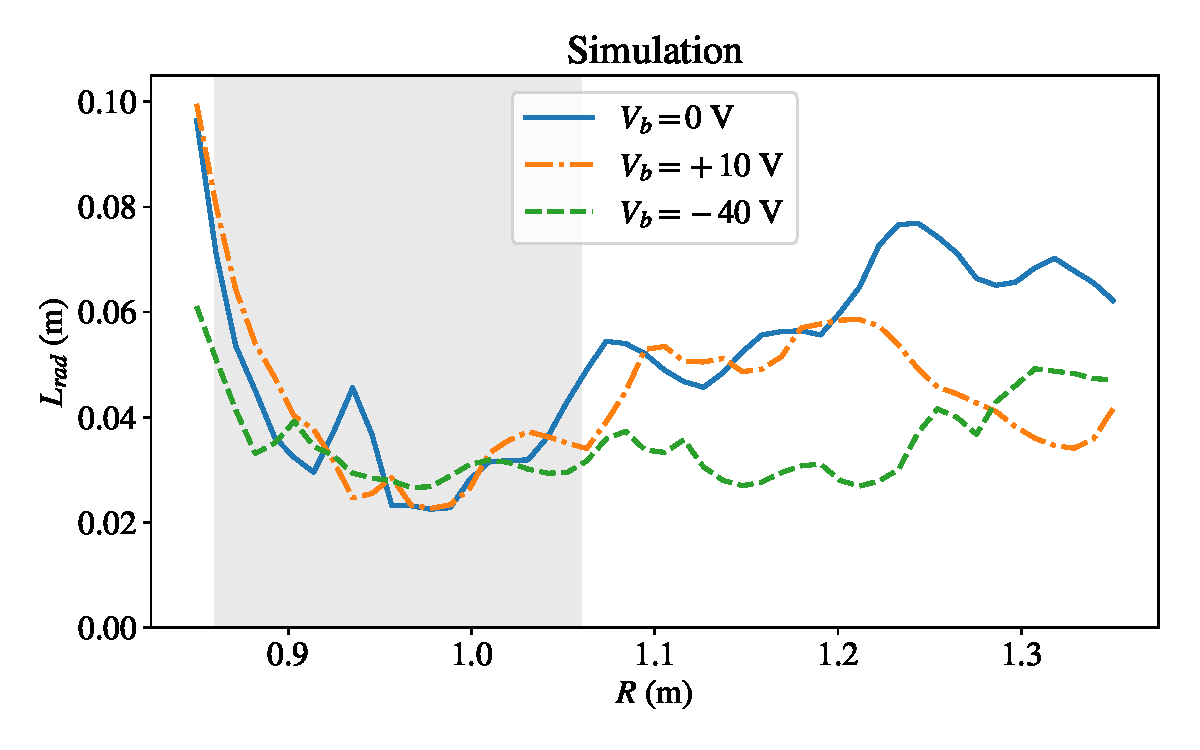
\includegraphics[width=.25\linewidth]{figs/lrad_Lc40_sim.pdf}
        %\caption{Caption}
        \label{fig:my_label}
    \end{figure}
    \vspace{-.75cm}
    \begin{figure}
        Experiment \\
        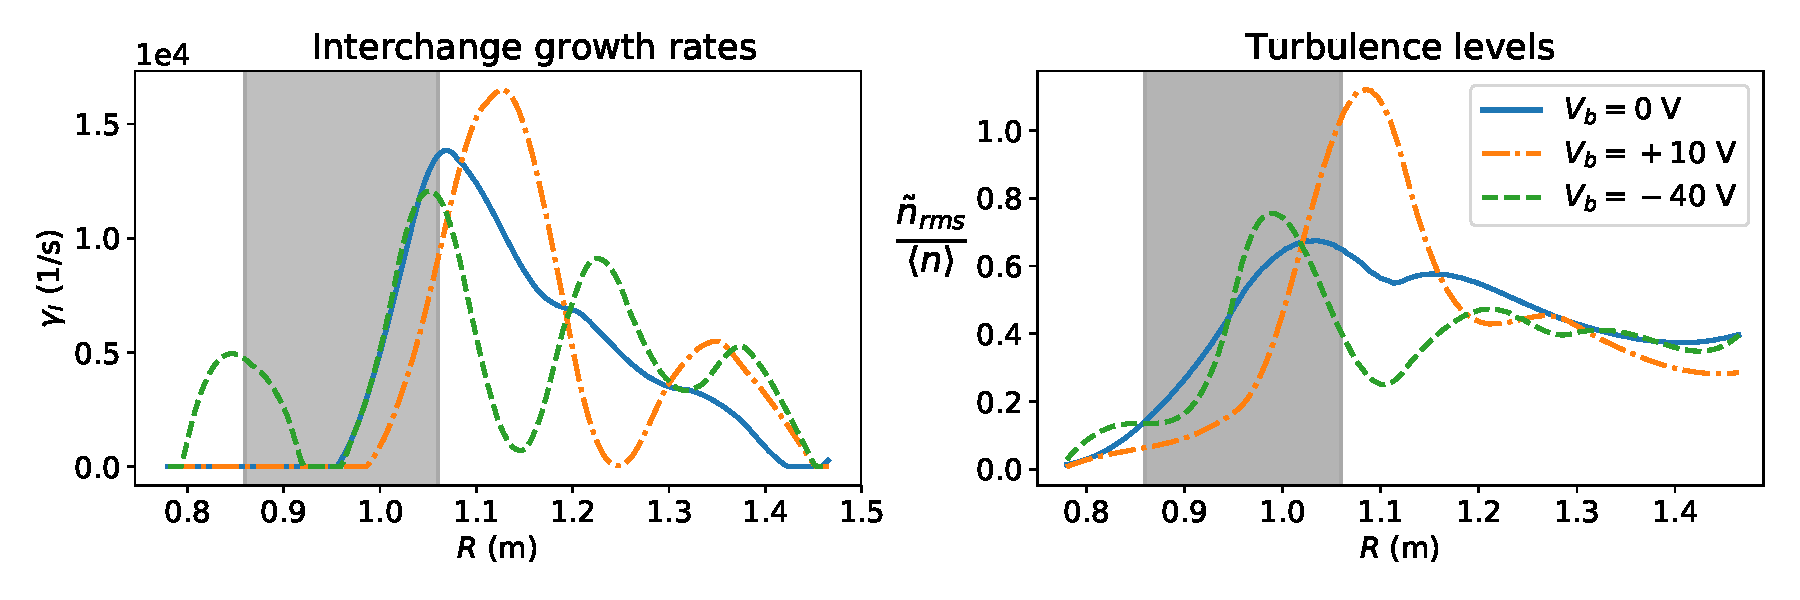
\includegraphics[width=.9\linewidth,left]{figs/gamma-dn-exp.pdf}
        %\caption{Caption}
        \label{fig:my_label}
    \end{figure}
\end{frame}

\begin{frame}{Shear may reduce radial correlation length in simulation}
    \begin{minipage}{.5\linewidth}
        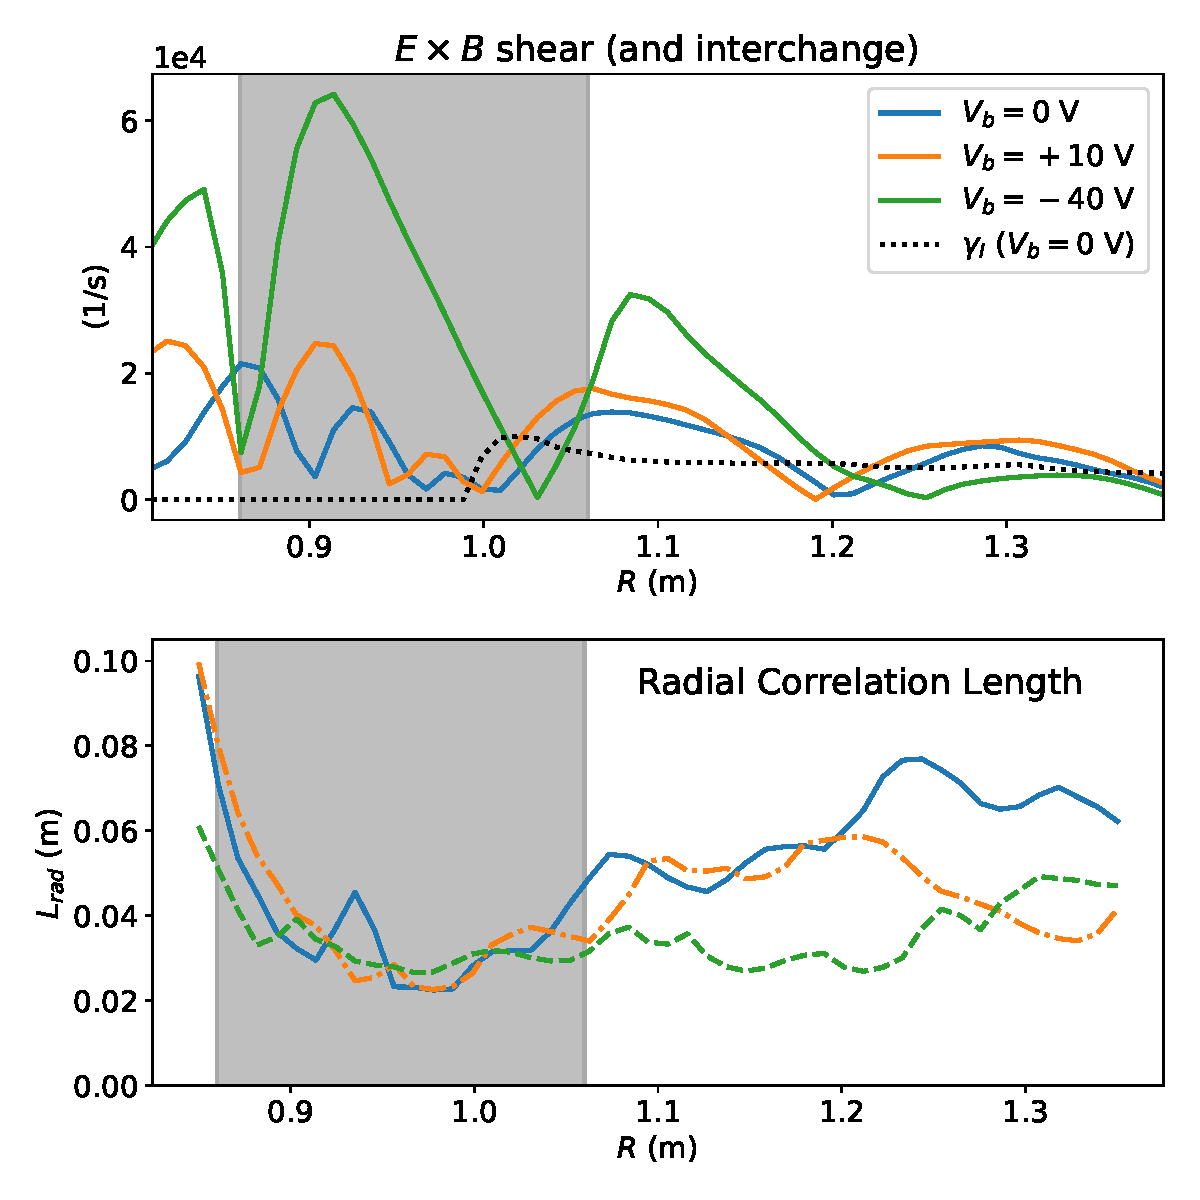
\includegraphics[width=\linewidth]{figs/lrad-comp-sim.pdf}
    \end{minipage}%
    \begin{minipage}{.49\linewidth}
    \begin{itemize} \footnotesize
        \item Radial correlation lengths appear reduced where shear in bad-curvature region ($R > 1.0$ m) is large.
        \item Turbulence levels, however, are not changed in bad-curvature region.
        \item Analysis of Kelvin Helmholtz modes suggested they are not present
        \begin{itemize} \footnotesize
            \item Condition for KH modes: $k_{min}\Delta_V  < \mathcal{O}(1)$ not satisfied
        \end{itemize}
    \end{itemize}
    \end{minipage}
\end{frame}

\section{Summary and future directions}
\begin{frame}{Outline}
    \tableofcontents[currentsection] 
\end{frame}

\begin{frame}{Conclusions}
    Grounded simulation ($V_b = 0$)
    \begin{itemize} \footnotesize
        \item Captured key features of experimental profiles
        \item Turbulence statistics show features of intermittency
        \item Small kinetic effects at the sheath
        \item Features such as vertical $E \times B$ flow, magnetic shear, and real electron mass likely necessary to improve agreement
    \end{itemize}
    Limiter-biased simulations
    \begin{itemize} \footnotesize
        \item Vertical $E \times B$ may be necessary for more accurate comparison
        \item Limiter-biasing changed bulk transport $\rightarrow$ changed equilibrium profiles ($n$) $\rightarrow$ changed linear growth rates and turbulence levels
        \item May explain why shear in the Helimak does not consistently reduce turbulence levels%\footnote{\scriptsize Gentle \etal, (2014)}
        \item Kelvin-Helmholtz modes likely not present
    \end{itemize}
    {\bf \small These results represent an important milestone in the effort to develop a self-consistent and computationally efficient gyrokinetic model of a tokamak SOL.}
\end{frame}

\begin{frame}{Future research}
    \begin{itemize}
        \item New version of \gke\ is $\sim$10x faster and includes new features
        \begin{itemize}
        \item Faster code for use of {\bf real electron mass} and {\bf non-linear Poisson equation}
        \item Includes {\bf magnetic shear} and {\bf vertical $\bm{E}\times \bm{B}$ flow}
        \item Conservative algorithms implemented for Fokker-Planck collision operator
        \item Symplectic formulation of electromagnetic fluctuations
        \end{itemize}
        \item Further developments are necessary
        \begin{itemize}
            \item Include radiation in source model
            \item Include neutral species in the model
            \item Improve BCs: account for non-normal $B$ at sheath
        \end{itemize}
        \item Carry out more detailed fluid--kinetic comparison
    \end{itemize}
\end{frame}

\begin{frame}{Acknowledgements}
\begin{block}{}
    \begin{itemize}
        \item Supervisors: Phil Morrison (UT) and Greg Hammett (PPPL)
        \smallskip
        \item Other committee members: Fran\c cois Waelbroeck, Ken Gentle
        \smallskip
        \item Main collaborators: Ammar Hakim (PPPL), Eric Shi (PU/LLNL), Tim Stoltzfus-Dueck (PPPL)
        \smallskip
        \item Other collaborators: Mana Francisquez (MIT), Jimmy Juno (UMD),  Noah Mandell (PU)
        \smallskip
        \item Experimental data: Ken Gentle, Eddie Taylor, Chad Williams
        \smallskip
        \item Computational resources: David Hatch, Jason Tenbarge, Fran\c cois Waelbroeck
    \end{itemize}
    \end{block}
    %This work used the Extreme Science and Engineering Discovery Environment (XSEDE), which is supported by National Science Foundation grant number ACI-1548562. This work was supported by the U.S. Department of Energy SCGSR program under contract DE-SC0014664, by DOE Contract DE-FG02-04ER-54742, through the Institute of Fusion Studies at the University of Texas at Austin, and DOE contract DE-AC02-09CH11466, through the Princeton Plasma Physics Laboratory (PPPL). 
\end{frame}

\appendix
\begin{frame}{Gyrokinetics:~time scales in Helimak\footnote{Perez \etal\ (2006)} and $\bm{B}^*$}
    Electron plasma frequency: $\omega_{pe} = 1.79 \times 10^{10}$ 1/s\\
    Electron gyrofrequency: $\Omega_{ce} = 1.76 \times 10^{10}$ 1/s \\
    Ion plasma frequency: $\omega_{pi} = 6.6 \times 10^{7}$ 1/s\\
    Ion gyrofrequency: $\Omega_{ci} = 2.59 \times 10^{5}$ 1/s
    \\
    \vspace{1cm}
    In the gyrokinetic equation... 
    \begin{align}
    B_\parallel^* &= \bm{b} \cdot \bm{B}_\parallel^* \\ \bm{B}_\parallel^* &= \bm{B} +(Bv_\parallel/\Omega_s)\nabla \times \bm{b}
    \end{align}
\end{frame}

\begin{frame}{Convergence testing}
    \begin{figure}
    \centering
    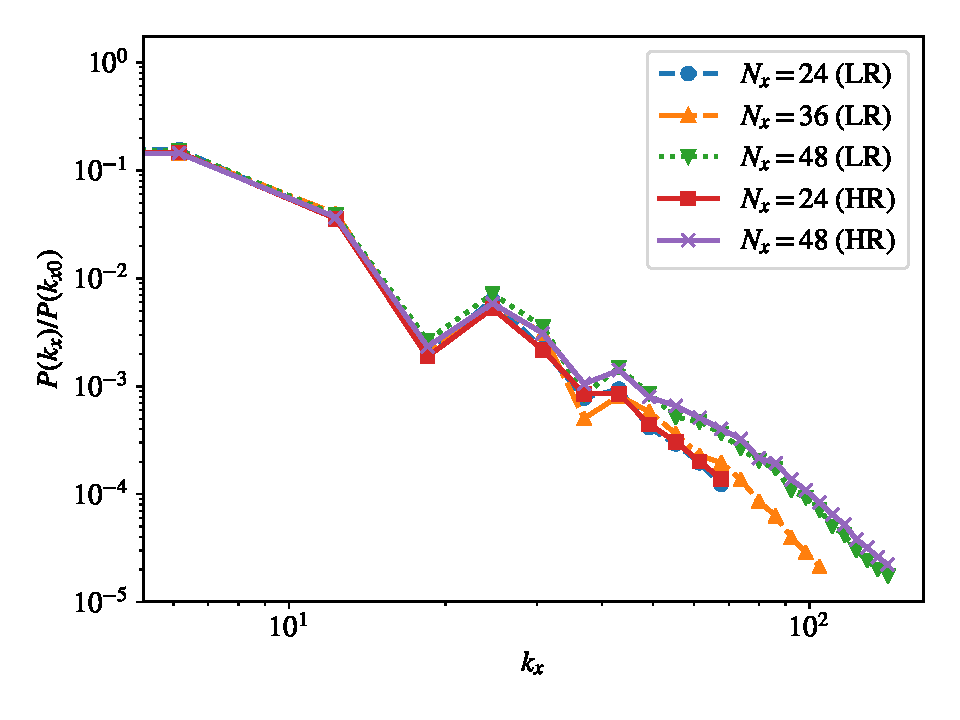
\includegraphics[width=.6\linewidth]{figs/kx-Nx-ths.pdf}
    \caption[Power in the Fourier transform in $x$ of electron density fluctuations compared for various resolutions.]{Power in the Fourier transform in $x$ of electron density fluctuations is compared for various resolutions. The power has been averaged in $y$, $z$, and in time from 10 to 16 ms. The low resolution case has $(N_x,N_y,N_z,N_{v_\parallel},N_\mu) = (N_x,12,8,10,5)$ and the higher resolution case has $(N_x,N_y,N_z,N_{v_\parallel},N_\mu) = (N_x,24,16,10,5)$. The decay of the power at high $k_x$ indicates that our simulations are not changed significantly with increased resolution.}
    \label{fig:kx-converge}
\end{figure}
\end{frame}

\begin{frame}{Radiation and neutral density}
    We estimated the total radiative cooling using the predicted radiative cooling rate $L_Z$ in Mavrin (2017). The total power radiated in the device is given by $P_{\text{rad}}\mathcal{V}= L_Z n_e n_{\text{imp}} \mathcal{V} \simeq 5.5$ kW, assuming $T_e = 10$ eV, $n_e=1 \times 10^{16}$ m$^{-3}$, and the total Argon density, including neutrals, is $n_{\text{imp}}=4 \times 10^{17}$ m$^{-3}$. $\mathcal{V}$ is the total volume of Helimak vacuum vessel.
\end{frame}

\begin{frame}{Real $m_e$}
    
\end{frame}

\begin{frame}{Bohm sheath criterion}
  Average $u_\parallel$ for ions compared with local $c_s$
  \begin{minipage}{.49\linewidth}
  \begin{figure}
      \centering
      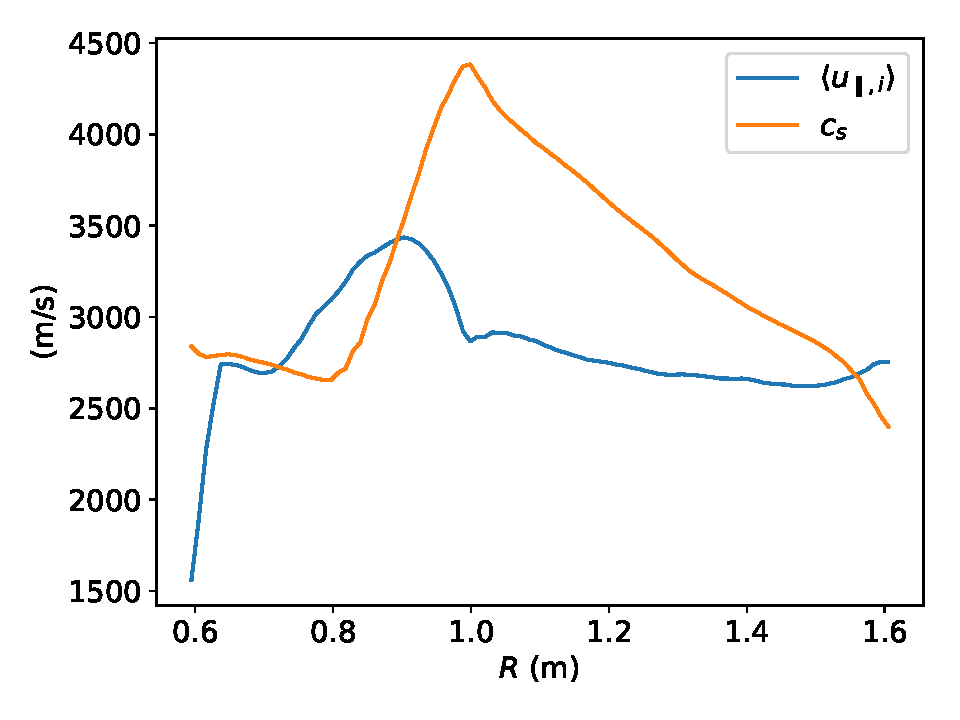
\includegraphics[width=\linewidth]{figs/cs-upar-T.pdf} \\
      \tiny Calculated at $z = L_z/2$
      \label{fig:my_label}
  \end{figure}
  \end{minipage}
    \begin{minipage}{.49\linewidth}
  \begin{figure}
      \centering
      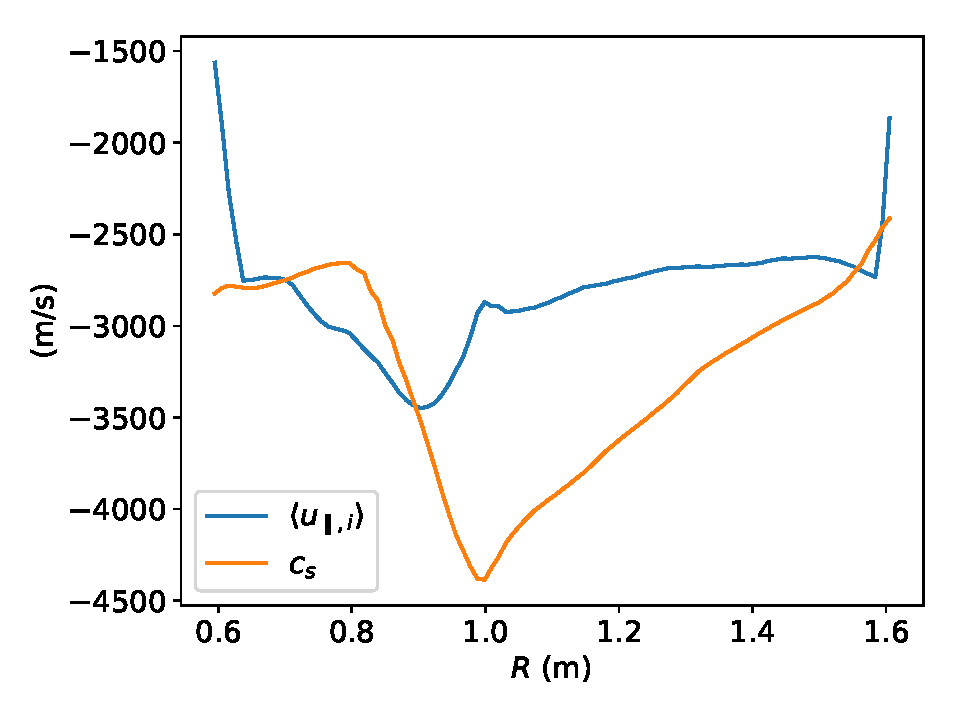
\includegraphics[width=\linewidth]{figs/cs-upar-B.pdf} \\
      \tiny Calculated at $z = -L_z/2$
      \label{fig:my_label}
  \end{figure}
  \end{minipage}
\end{frame}

\begin{frame}{Interchange growth rate derivation}
Begin with ArcOn equations:
    \begin{align}
    \partial_t n + [\phi, n ] = - \alpha n + D \nabla_\bot ^2 n + S_n \label{eq:arc-n}\\
    \partial_t U + [\phi, U ] =  \alpha \phi - \beta [x, \ln n] + \mu \nabla_\bot ^2 U \label{eq:arc-u}\\
    U = \nabla_\bot ^2 \phi, \label{eq:arc-phi}
\end{align}
Linearizing and substituting for $U$ gives
\begin{align}
-i \omega \tilde{n} - i k n_0' \tilde{\phi}  = - D k^2 \tilde{n} \\
i \omega k^2 \tilde{\phi} = \alpha \tilde{\phi} + i k \frac{\beta}{n_0} \tilde{n} + \mu k^4 \tilde{\phi}.
\end{align}
\end{frame}

\begin{frame}{Polarization current (and blobs)}
    Assuming quasineutrality, $\nabla \cdot (\bm{j}_d + \bm{j}_p) + \nabla_\parallel j_\parallel = 0$
    \begin{eqnarray}
    \bm{j}_d &=& (\bm{B}/B^2) \times \nabla p \\
    \bm{j}_p &=& (-n m_i / B^2)d_t\nabla \phi \\
    j_\parallel &=& en(V_{\parallel i} - V_{\parallel e}).
    \end{eqnarray}
    Using the Boussinesq approximation, $\nabla \cdot \bm{j}_p \approx (-nm_i / B^2) d_t \nabla^2 \phi$, and the divergence of the diamagnetic drift, $\nabla \cdot \bm{j}_d = \left ( \nabla \times \bm{B}/B^2 \right) \cdot \nabla p $ gives
    \begin{align}
    \frac{nm_i }{B^2} d_t \nabla^2 \phi &= \left ( \nabla \times \frac{\bm{B}}{B^2} \right ) \cdot \nabla p + \nabla_\parallel [en(V_{\parallel i} - V_{\parallel e})]
    % &= \left ( \frac{2\bm{b} \times \bm{\kappa}}{B}\right ) \cdot \nabla p + \nabla_\parallel [en(V_{\parallel i} - V_{\parallel e})],
    \end{align}
\end{frame}

\end{document}

% Backup slides / Questions
% Polarization current -- return current
% Interchange growth rate derivation
% Comparison of time scales in helimak
% Convergence testing
% KH stability analysis
% radiation and neutral density
% real m_e
% Be prepared to answer about B*, related to curvature drift and conservation (symplectic nature of Hamiltonian system??)



